\documentclass[11pt, twoside]{report}

\usepackage[T1]{fontenc}
\usepackage[utf8]{inputenc}
%%\usepackage[us]{babel}
\usepackage{helvet}
\usepackage[a4paper,width=180mm,top=20mm,bottom=20mm,bindingoffset=6mm]{geometry}
\usepackage[framemethod=default]{mdframed}
\usepackage{lipsum,titlesec,xcolor,fancyhdr,array,multicol,float,graphicx,wrapfig,subcaption}
\usepackage{fontspec,todonotes,enumitem,comment,capt-of,amsmath,booktabs}
\usepackage[colorlinks]{hyperref}
\usepackage[font=scriptsize]{caption}
\usepackage[sorting=none]{biblatex}
\addbibresource{references.bib}


\DeclareCaptionLabelFormat{andtable}{#1˜#2 \& \tablename˜\thetable}

\renewcommand{\familydefault}{\sfdefault}

\graphicspath{{images/}}

%% define size for chapter initial page:
\usepackage{titlesec, blindtext, color}
\definecolor{gray75}{gray}{0.75}
\newcommand{\hsp}{\hspace{20pt}}
\titleformat{\chapter}[hang]{\Huge\bfseries}{\thechapter\hsp\textcolor{gray75}{|}\hsp}{0pt}{\Huge\bfseries}

\titlespacing*{\chapter}{0pt}{-60pt}{20pt} %% change spacing

\usepackage{enumitem}
\setlist{noitemsep}
%%%%%%%%%%


\floatstyle{plain}
\restylefloat{figure}

\pagestyle{fancy}
\fancyhf{}
\renewcommand{\chaptermark}[1]{ \markboth{#1}{} }
\renewcommand{\sectionmark}[1]{ \markright{#1}{} }
\fancyhead[LE]{\itshape{ \fontsize{10}{12} \selectfont \leftmark}}
\fancyhead[RE, LO]{\thepage}
\fancyhead[RO]{\itshape{\fontsize{10}{12} \selectfont \rightmark}}
\renewcommand\headrulewidth{0pt}

 \hypersetup{
     colorlinks,
     citecolor= green,
     filecolor= black,
     linkcolor= black,
     urlcolor= blue
 }

\usepackage[nottoc,notlot,notlof]{tocbibind}
 
\begin{document}
    \begin{titlepage}
    \centering
    
\includegraphics[width=0.30\textwidth]{images/cherubino_black.pdf}\par\vspace{1cm}
    {\scshape\LARGE Università di Pisa \par}
    \vspace{1cm}
    {\scshape\ Social Network Analysis \\A.A. 2017/2018\par}
    \vspace{1.5cm}
    {\huge\bfseries Cambridge Analytica and Facebook: \\ The Scandal and the Fallout on Twitter\\ \par}
    \vspace{2cm}
    {\Large Gianmarco Ricciarelli 555396 \\ Stefano Carpita 304902 \par}
    \vfill

\begin{flushright}    
  \textit{Data drives all we do.}\\
\vspace{2 mm}
Cambridge Analytica main slogan.
\end{flushright}

\vspace{4 mm}
    
\begin{flushright}    
  \textit{Rules don’t matter for them. \\ For them, this is a war, and it’s all fair.}\\
\vspace{2 mm}
  Christopher Wylie, \\ former datascientist at Cambridge Analytica, about its leaders.
\end{flushright}




  \end{titlepage}


    \pagenumbering{Roman}
    \tableofcontents
    \chapter{The case story}
    \pagenumbering{arabic}

On Saturday $17^{th}$ of March 2018, The New York Times and The Guardian / The Observer broke reports on how the consulting firm Cambridge Analytica harvested private information from the Facebook profiles of more than 50 million users without their permission, making it one of the largest data leaks in the social network’s history. \cite{guardian}, \cite{nyt_17march}.

Cambridge Analytica described itself as a company providing consumer research, targeted advertising and other data-related services to both political and corporate clients.

The whistleblower Christopher Wylie, datascientist and former director of research at Cambridge Analytica revealed to the Observer how Cambridge Analytica used personal information taken without authorisation in early 2014 to build a system that could profile individual US voters, in order to target them with personalised political advertisements.
Christopher Wylie, who worked with a Cambridge University academic to obtain the data, told the Observer: “We exploited Facebook to harvest millions of people’s profiles. And built models to exploit what we knew about them and target their inner demons. That was the basis the entire company was built on.”

What, Where, Who, Why, Where ?


Timeline da sistemare: \cite{nyt_timeline}
\begin{itemize}

\item March 17, 2018: The Observer and The New York Times publish joint reports on data harvesting by Cambridge Analytica. UK Information Commissioner Elizabeth Denham issues statement that they are “investigating circumstances in which Facebook data may have been illegally acquired and used.” Politicians in US and UK call for investigation.

\item March 19, 2018: Channel 4 News publishes part 1 of their undercover investigation into Cambridge Analytica. Facebook sends investigators to Cambridge Analytica’s offices. UK Information Commissioner orders them to stand down.

\item March 20, 2018: Channel 4 News publishes part 2 of their undercover investigation into Cambridge Analytica, where they boast about getting Donald Trump elected. British MP Damian Collins calls on Facebook to present oral evidence on Cambridge Analytica. Facebook agrees to send former operations manager Sandy Parakilas. Facebook holds internal Q\&A with attorney Paul Grewal to discuss the crisis, but CEO Mark Zuckerberg and COO Sheryl Sandberg do not attend. Cambridge Analytica suspends CEO Alexander Nix. Facebook demands to inspect Christopher Wylie’s phone. FTC opens investigation into Facebook.
\item to be continued...
\end{itemize}

    \chapter{Building the network}
    In this report we present an analysis of the spreading of the Cambridge Analytica-Facebook scandal on Twitter.
    We have considered a network composed by the authors of tweets about the case, during the first period of the scandal outbreak. The data have been collected via the Twitter API and we built the network using the following consecutive steps:
    \begin{enumerate}
    \item Crawling of all the available tweets over a period of more than 15 days, since the $17^{th}$ of March, containing at least one of the most popular hashtags regading the case:\\
    \textbf{  \{\#cambridgeanalytica, \#facebookgate, \#deletefacebook, \#zuckerberg \} }
      
    \item Cleaning of the crawled tweets, by selecting and storing in a MongoDB database only the users informations about the authors of tweets, excluding retweets and mentions.
    \item Selection of the case outbreak time period by observing the time history in Fig. \ref{fig:time_history}. The selected time period consists of 8 days, from the $17^{th}$ to the $24^{th}$ of March included (considering the Italian timezone). 
      
    \item Crawling of the following list for each of the selected authors, extracting the followee/follower relationships.
    \end{enumerate}
    In Fig. \ref{fig:time_history} is represented the rate of new authors per hour. %%In the weekend of $17^{th}$ $18^{th}$
    We can observe a tipical daily periodicity, with peaks during the Italian afternoon, corresponding to the USA waking up.
    The first relevant rate increase is observed on the Monday $19^{th}$, following the weekend of news publishing. A stationary evolution is observed after the $24^{th}$ of March, a week after the scandal outburst.
    %%Relevant peaks are in correspondance on major events likewise...

    The collecting of the following lists of all the authors has been necessary in order to overcome the huge time complexity of a direct crawling of the
    followee/follower relationships, considering also the Twitter API rates limits. A negligible fraction of the following lists was not available, because of the Twitter privacy settings of the users.

    In summary, we built a directed unweighted network, consisting of:

    \begin{itemize}
    \item \textbf{Nodes}: $65729$ twitter users, authors of tweets containing at least one of the hashtags specified above.

    \item \textbf{Edges}: $2501757$ followee/follower relationships between the selected authors.
    \end{itemize}


    
    \begin{figure}[htbp]
      \centering
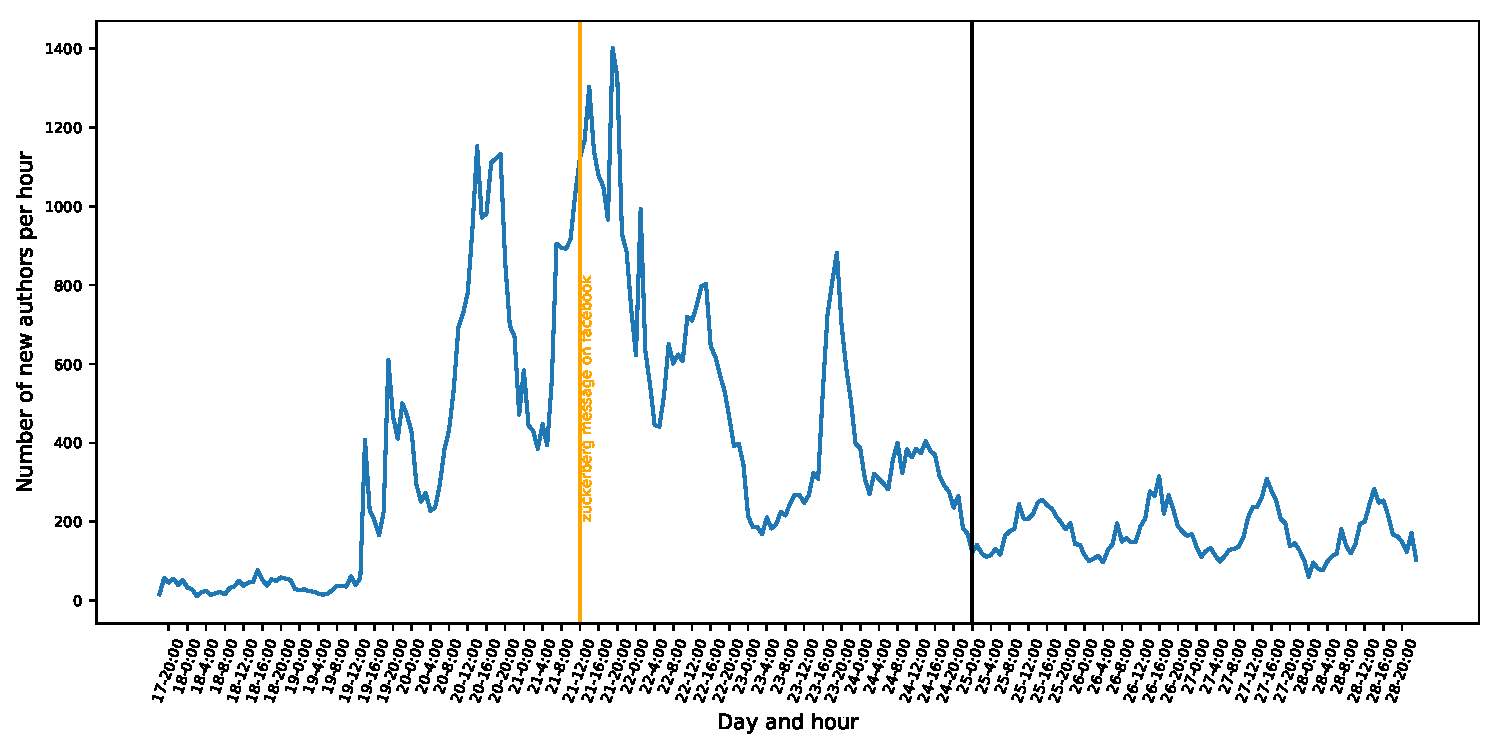
\includegraphics[width=\textwidth]{../../scripts/network_analysis/imgs/time_history.pdf}
      \caption{Time history of the rate of new authors per hour, during the first 12 days from the first publishing of the scandal.}
      \label{fig:time_history}
    \end{figure}



    
    \chapter{Network analysis}

\section{Network properties summary} 

\begin{table}[htbp]
  \centering
\begin{tabular}{lllll}
\toprule
{} &        g &    g\_und &     g\_er &     g\_ba \\
\midrule
L         &  2501757 &  1895878 &  4318406 &  4989628 \\
N         &    65729 &    65729 &    65729 &    65729 \\
density   &  0.00058 &  0.00088 &    0.001 &  0.00231 \\
gamma     &      2.6 &     None &     None &      2.9 \\
gamma\_in  &      2.4 &     None &     None &     None \\
gamma\_out &      2.9 &     None &     None &     None \\
gamma\_tot &      2.6 &     None &     None &     None \\
k\_avg     &       38 &       57 &       65 &      151 \\
k\_in\_max  &    19064 &     None &      109 &     None \\
k\_in\_min  &        0 &     None &       36 &     None \\
k\_max     &    19073 &    19065 &      183 &     3640 \\
k\_min     &        1 &        1 &       84 &       76 \\
k\_out\_max &     4130 &     None &      103 &     None \\
k\_out\_min &        0 &     None &       35 &     None \\
\bottomrule
\end{tabular}

\end{table}

\subsection{Random graphs}

The network has been compared throughout the report with two synthetic network, an Erdos-Renyi random network and a Barabasi-Albert network.
The Erdos-Renyi random network, with directed connections, has been generated with a value of the ``linking probability'' $p$ computed using the double of the average degree of the original network:
    \begin{equation}
      p_{ER} \approx \frac{2\langle k  \rangle}{N} = \frac{76}{65729} \approx  0.001
      \label{eq:ER_probability}
    \end{equation}

 An undirected network built with the Barabasi-Albert model  has an average degree equal to the double of the links formed by each new node: $ \, \langle k_{BA} \rangle = 2 m$ \cite{network_science}. Because our network is directed we generated a Barabasi-Albert random network with a value of $m$ equal to half of the double of the average degree of the original network, or simply equal to the average degree of our directed graph:
    \begin{equation}
      m = \frac{ 2 \, \langle k \rangle}{2} =  \langle k \rangle = 38
      \label{eq:BA_model}
    \end{equation}

    
 \section{Degree distribution}    

 
\begin{minipage}[b]{0.5\textwidth}
   \centering
    \begin{figure}[H]
      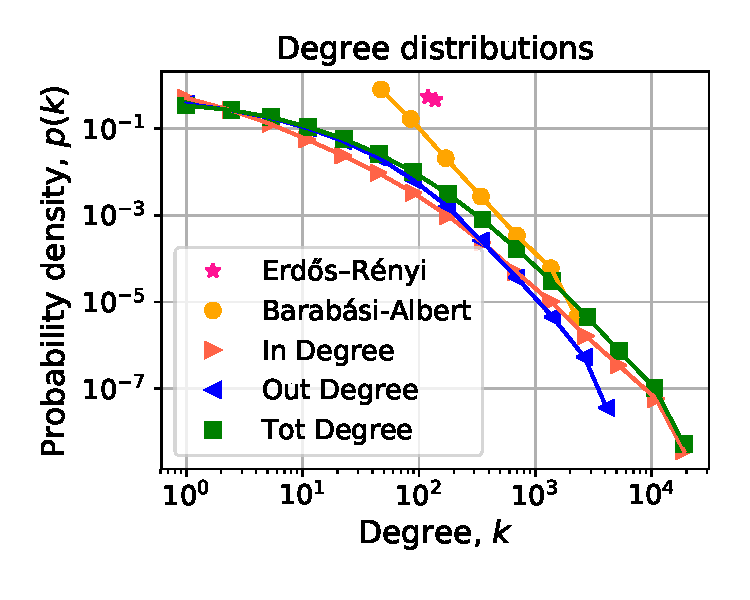
\includegraphics[width=\textwidth]{../../scripts/network_analysis/imgs/degree_distributions.pdf}            
          \caption{}
        \label{fig:in_degree}
\end{figure}
\end{minipage}
\begin{minipage}[b]{0.5\textwidth}
  \begin{figure}[H]
  \centering
  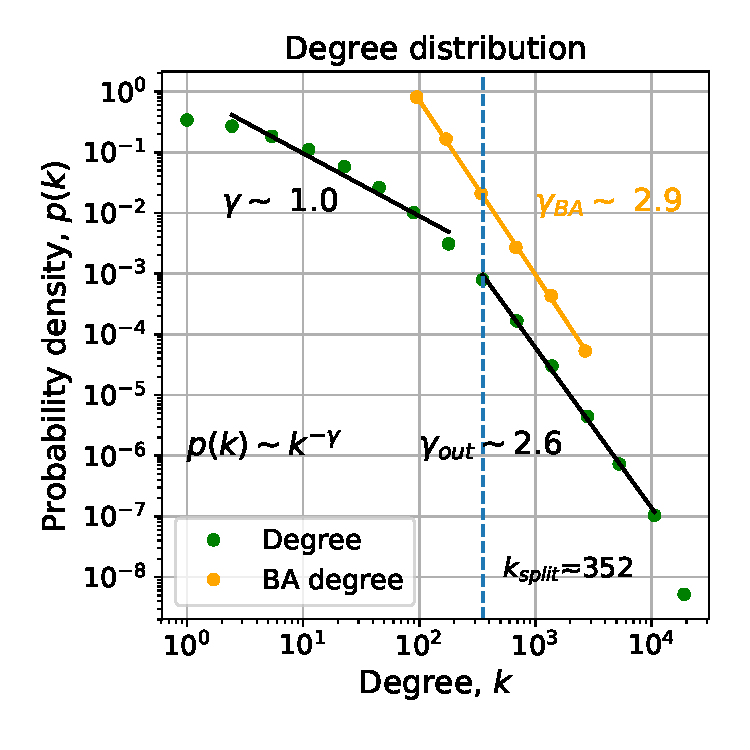
\includegraphics[width=\textwidth]{../../scripts/network_analysis/imgs/tot_degree_distribution.pdf}            
        \caption{}
\label{fig:out_degree}
\end{figure}
\end{minipage}
    
\begin{minipage}[b]{0.5\textwidth}
   \centering
    \begin{figure}[H]
      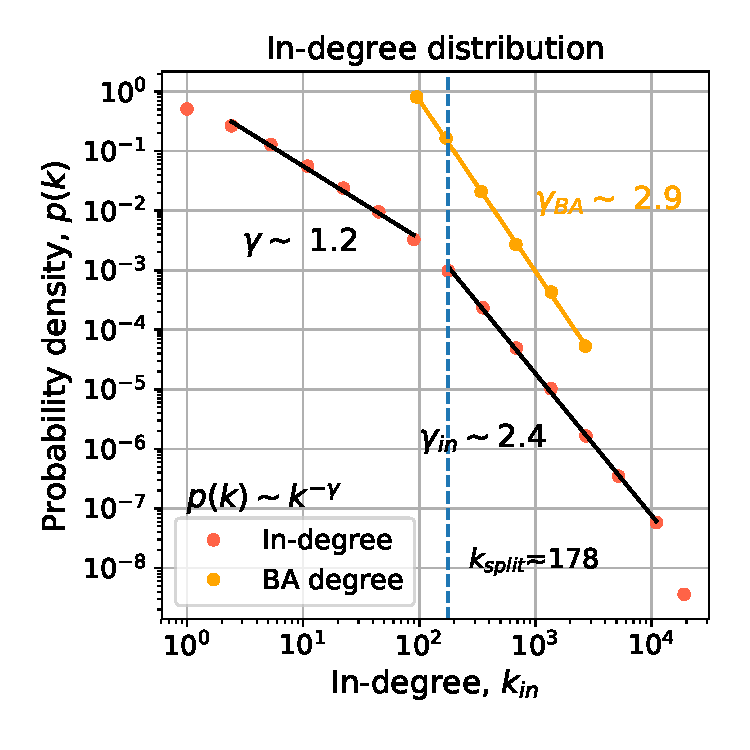
\includegraphics[width=\textwidth]{../../scripts/network_analysis/imgs/in_degree_distribution.pdf}            
          \caption{}
        \label{fig:in_degree}
\end{figure}
\end{minipage}
\begin{minipage}[b]{0.5\textwidth}
  \begin{figure}[H]
  \centering
  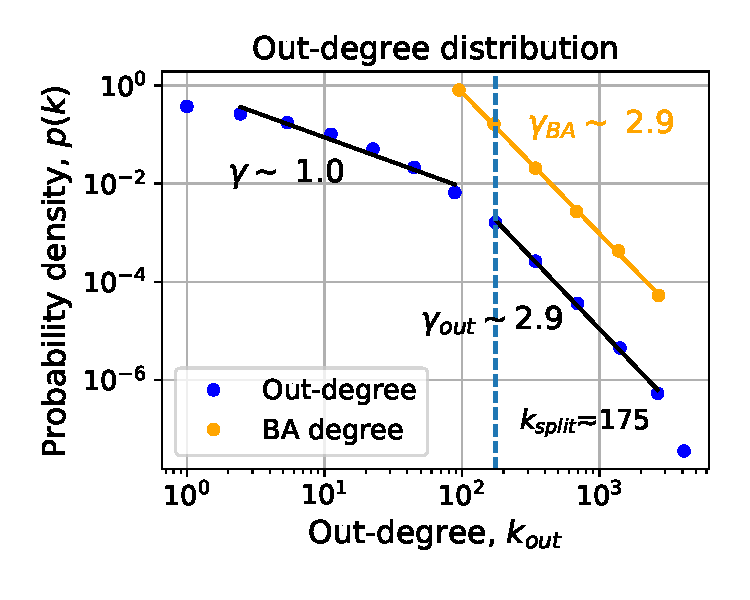
\includegraphics[width=\textwidth]{../../scripts/network_analysis/imgs/out_degree_distribution.pdf}            
        \caption{}
\label{fig:out_degree}
\end{figure}
\end{minipage}

 \begin{figure}[htbp]
      \centering
      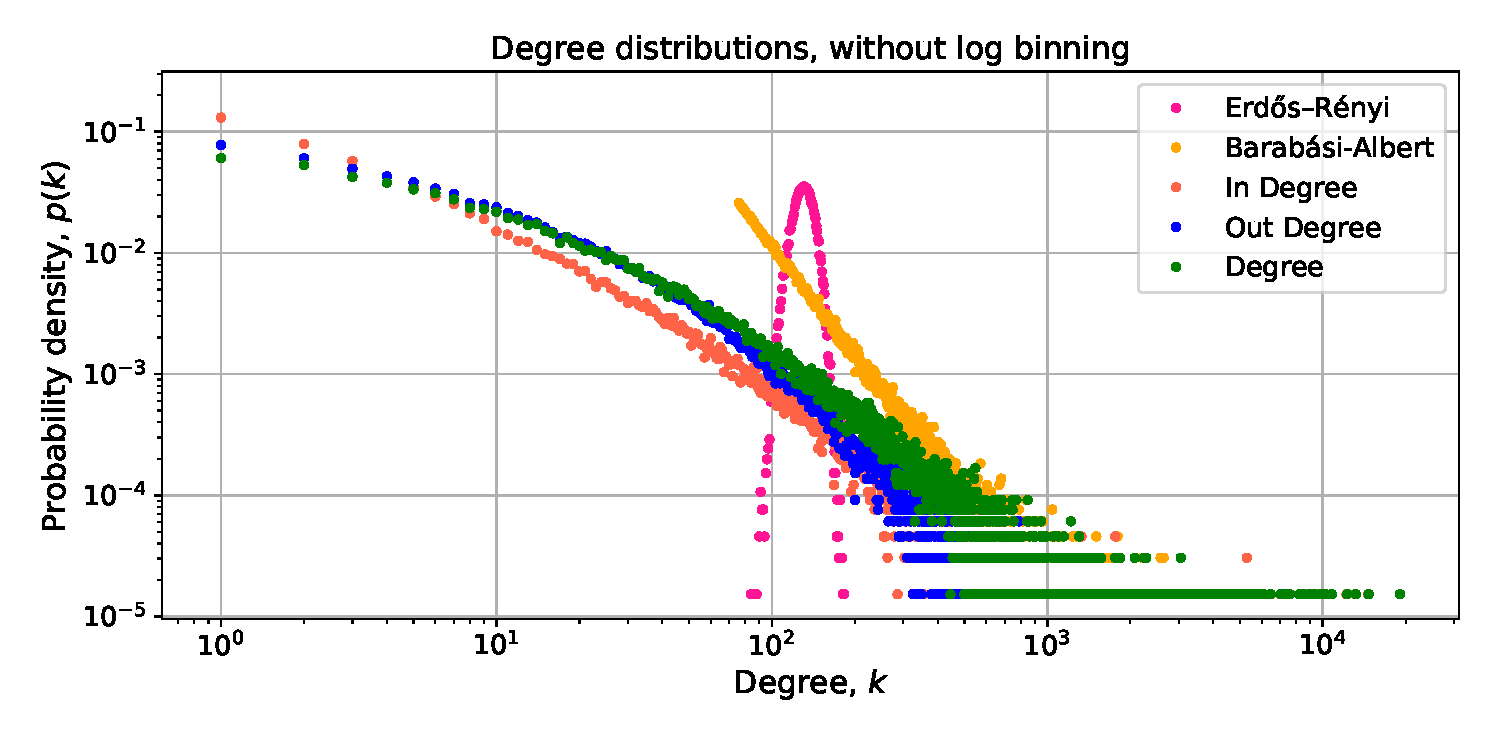
\includegraphics[width=0.8\textwidth]{../../scripts/network_analysis/imgs/degree_distributions_nobinlog.pdf}            
      \caption{New authors time history}
      \label{fig:degree}
    \end{figure}



    
    \begin{figure}[htbp]
      \centering
      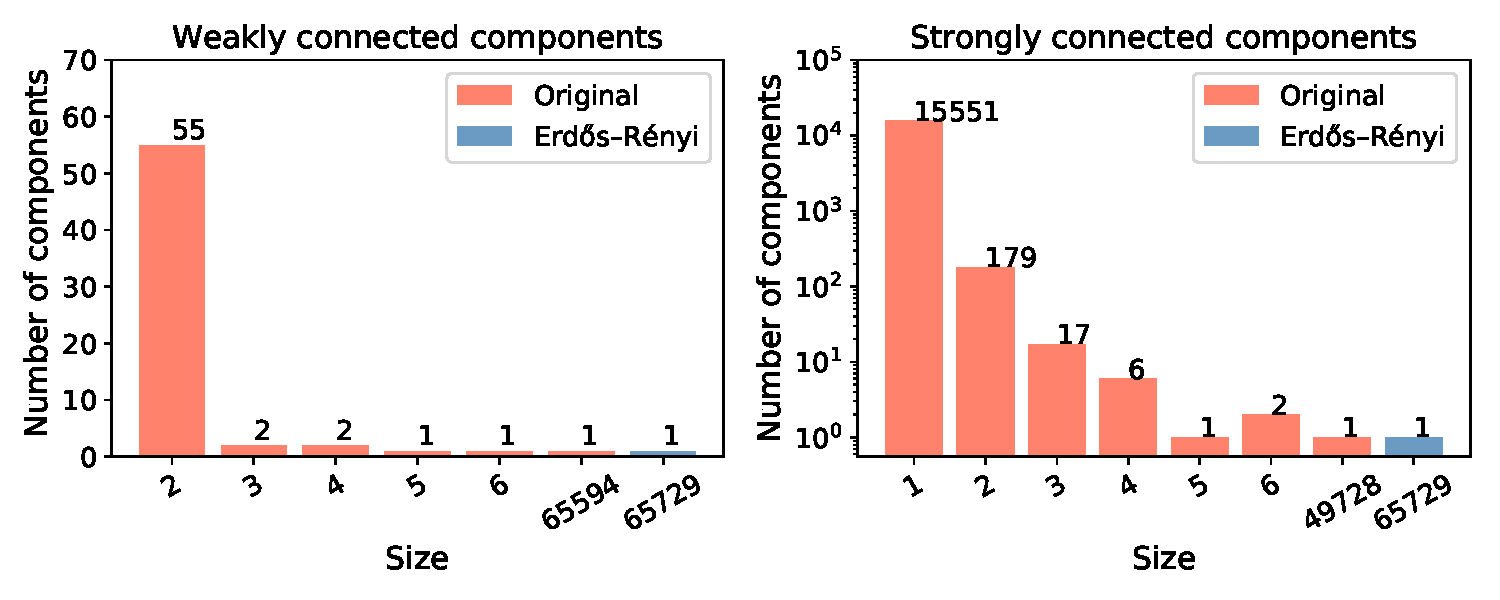
\includegraphics[width=\textwidth]{../../scripts/network_analysis/imgs/connectivity.pdf}            
      \caption{Connect components}
      \label{fig:connectivity}
    \end{figure}


    \section{Path analysis}
    In order to exactly estimate the average path length $\langle d \rangle$ it would be necessary to compute all the node-node distances of the network. These procedure results infeasible with the computation resources available, as shown in Fig. \ref{fig:path_time}.
    In real networks the path length distribution is quite close to a normal distribution, as shown in \cite{ye_paths}. The average path length has then been estimated statistically, random sampling a number $n$ of node pairs, sufficient to achieve a narrow confidence interval for the mean. The assumption of normality of the distribution it is strong, but not necessary. The convergence of the computed mean to the expected value is guaranteed by the central limit theorem with the assumptions that the distances are independent, identically distributed, and with finite variance.
    The average path length has been estimated by the average of the distances $D_i$ for each sampled node pair, and computing its standard deviation:
    \begin{equation}
      \langle d \rangle = \frac{\sum D_i}{n} \; , \; \sigma(\langle d \rangle) = \frac{s}{\sqrt{n}}
    \end{equation}


    
\begin{minipage}[b]{0.5\textwidth}
   \centering
    \begin{figure}[H]
      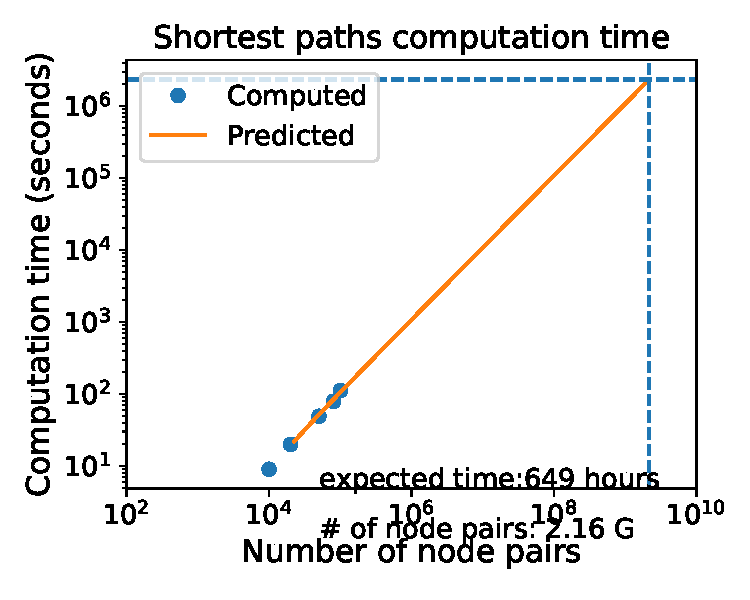
\includegraphics[width=\textwidth]{../../scripts/network_analysis/imgs/paths_computation_time.pdf}            
          \caption{Shortest paths computation time by number of pairs}
      \label{fig:path_time}
\end{figure}
\end{minipage}
\begin{minipage}[b]{0.5\textwidth}
  \begin{figure}[H]
  \centering
      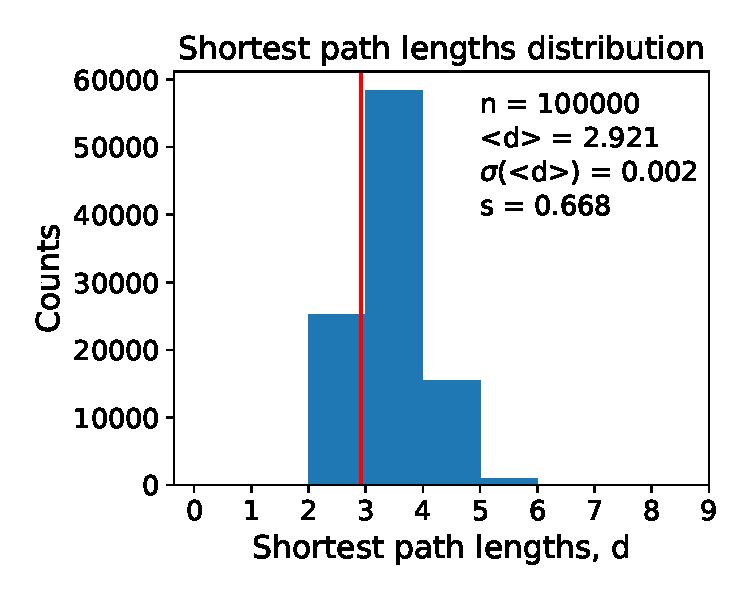
\includegraphics[width=\textwidth]{../../scripts/network_analysis/imgs/paths_hist.pdf}            
        \caption{Shortest paths distribution}
\end{figure}
\end{minipage}

    
    \begin{figure}[htbp]
      \centering
      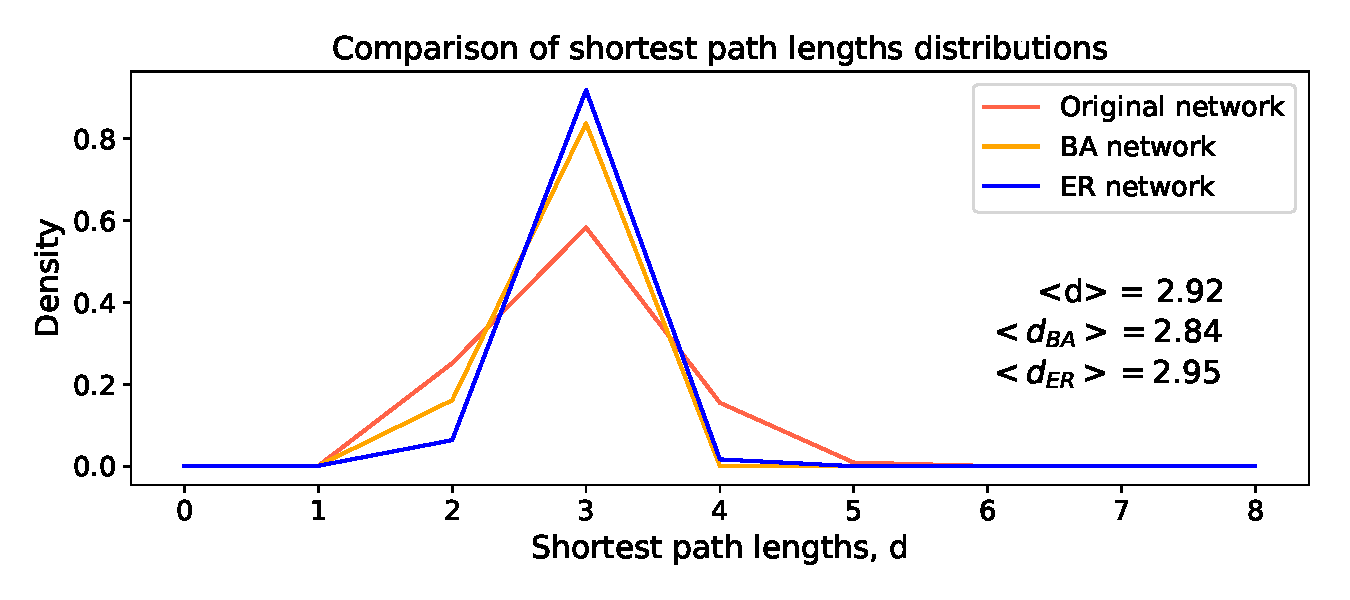
\includegraphics[width=\textwidth]{../../scripts/network_analysis/imgs/paths_hist_comparison.pdf}            
      \caption{Shortest paths distributions comparison between the original undirected graph and the random networks.}
      \label{fig:path_comparison}
    \end{figure}



\begin{minipage}[b]{0.5\textwidth}
   \centering
    \begin{figure}[H]
      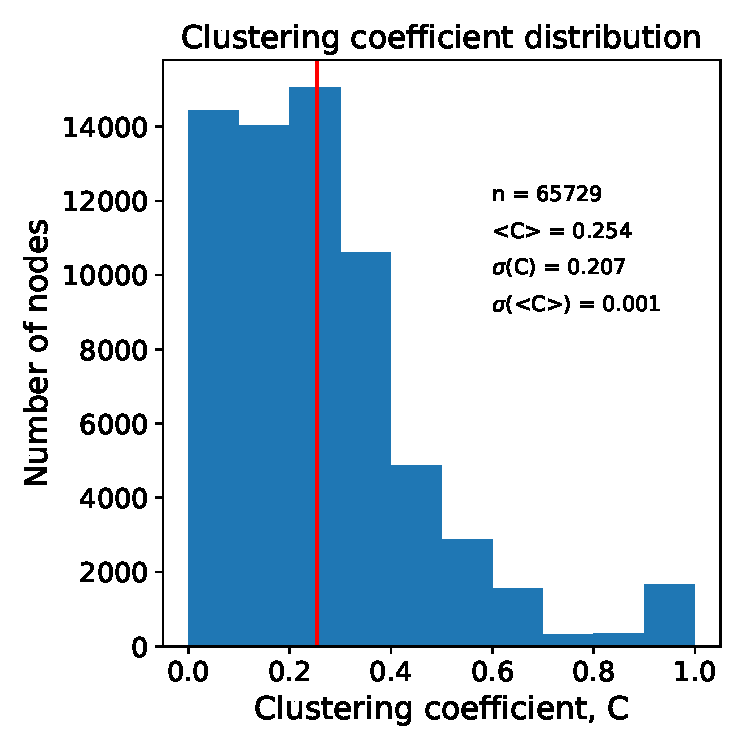
\includegraphics[width=\textwidth]{../../scripts/network_analysis/imgs/cluster_coef_hist.pdf}            
          \caption{Clustering coefficient distribution}
      \label{fig:path_time}
\end{figure}
\end{minipage}
\begin{minipage}[b]{0.5\textwidth}
  \begin{figure}[H]
  \centering
      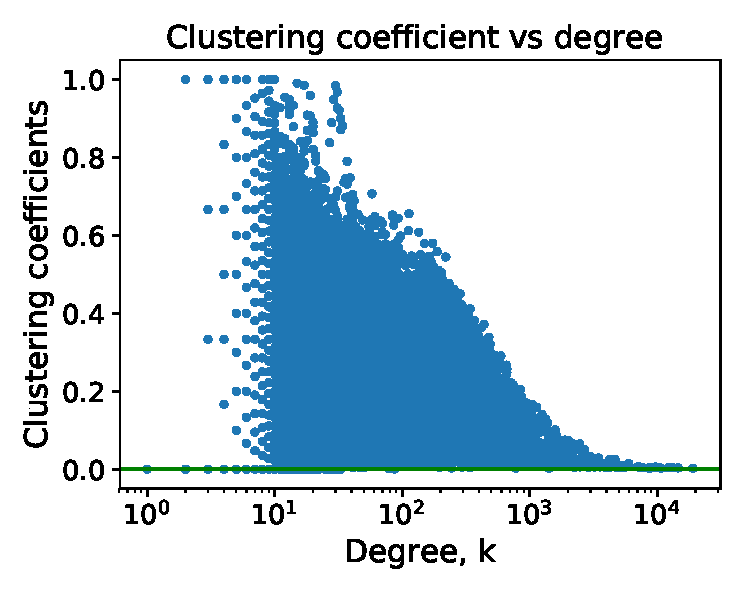
\includegraphics[width=\textwidth]{../../scripts/network_analysis/imgs/cluster_coef_bydegree.pdf}            
      \caption{Clustering coefficients as function of the degree}
\end{figure}
\end{minipage}

\clearpage
\section{Hubs analysis}

The hubs of the crawled social network of tweets authors about the Cambridge Analytica-Facebook scandal are mainly
news mass media, as expected. In Fig. \ref{fig:hubs_followers} the 30 biggest hubs are represented by indicating
the in-degree of the crawled network, corresponding to the number of authors following the hub, versus the actual total
number of followers on Twitter.
The "The New York Times" is the biggest hub, with the maximum number of both in-degree and number of followers.
We observe that there is an obvious positive correlation between in-degree and followers, with some variations.
In particular, let's take a pair of hubs having similar followers count, such as the "Washington Post" and the "Huffington Post".
The "Washington Post" has a larger in-degree than the second.
This difference can be interpreted as a larger interest in the scandal from the people following the "Washington Post'' respect 
to the ones following the "Huffington Post".
We can define a quantity to measure this interest:

\begin{equation}
  \text{Interest} \equiv \frac{ \text{in-degree} }{\text{\#followers}}
  \label{eq:interest}
\end{equation}

This measure represents the percentage of followers that being interested in the scandal had published a tweet about the subject.
%%It is also a measure of density, being the analyzed network a sub-network of the overall Twitter network: 



    \begin{figure}[htbp]
      \centering
      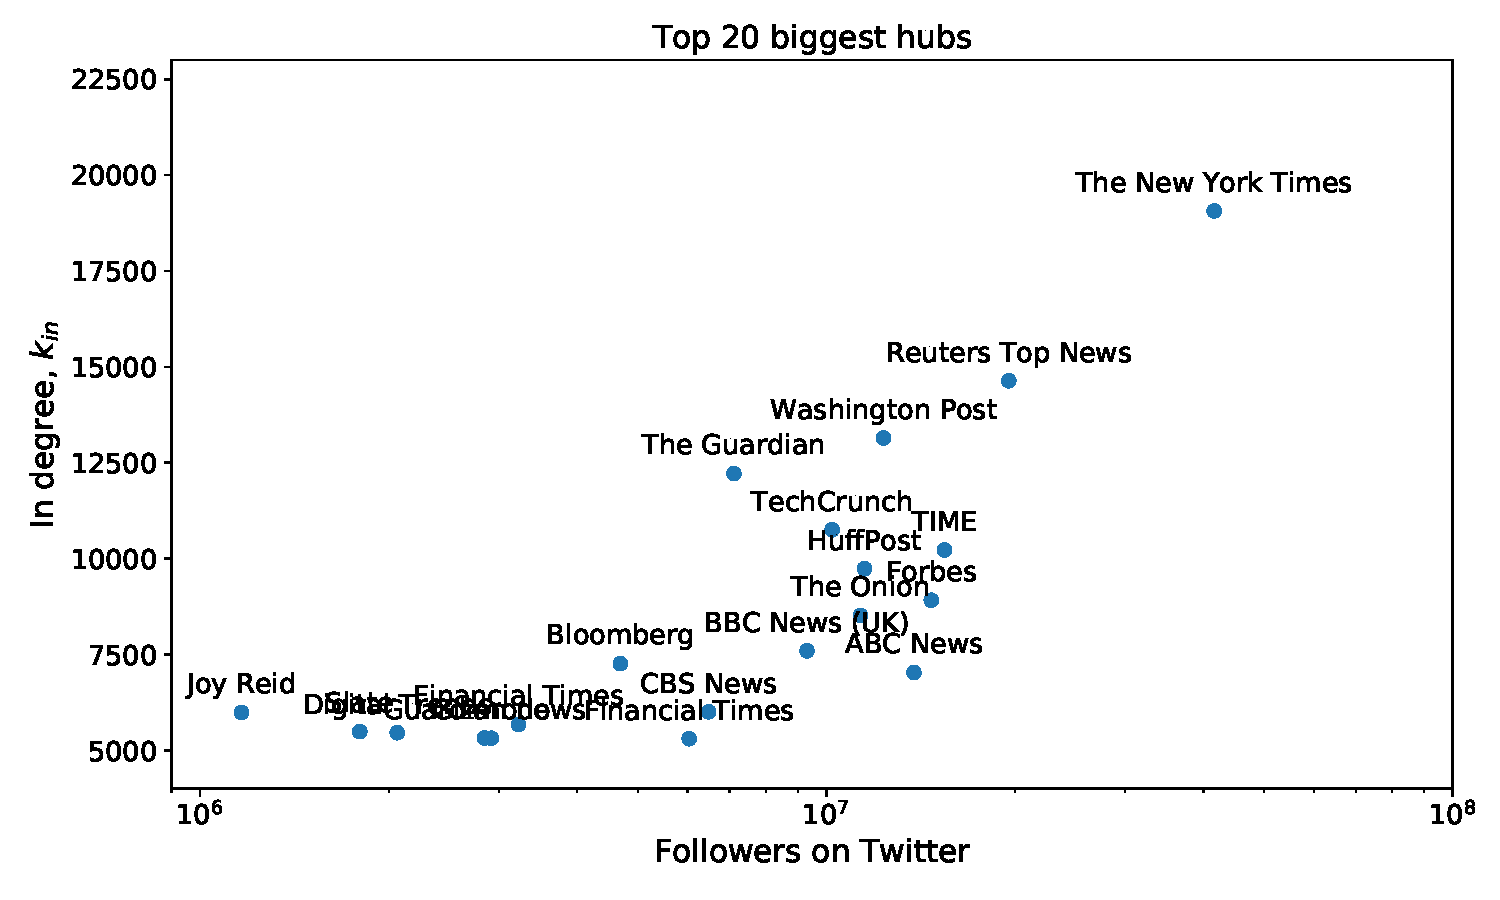
\includegraphics[width=\textwidth]{../../scripts/network_analysis/imgs/hubs_followers.pdf}            
      \caption{}
      \label{fig:hubs_followers}
    \end{figure}

    \begin{figure}[htbp]
      \centering
      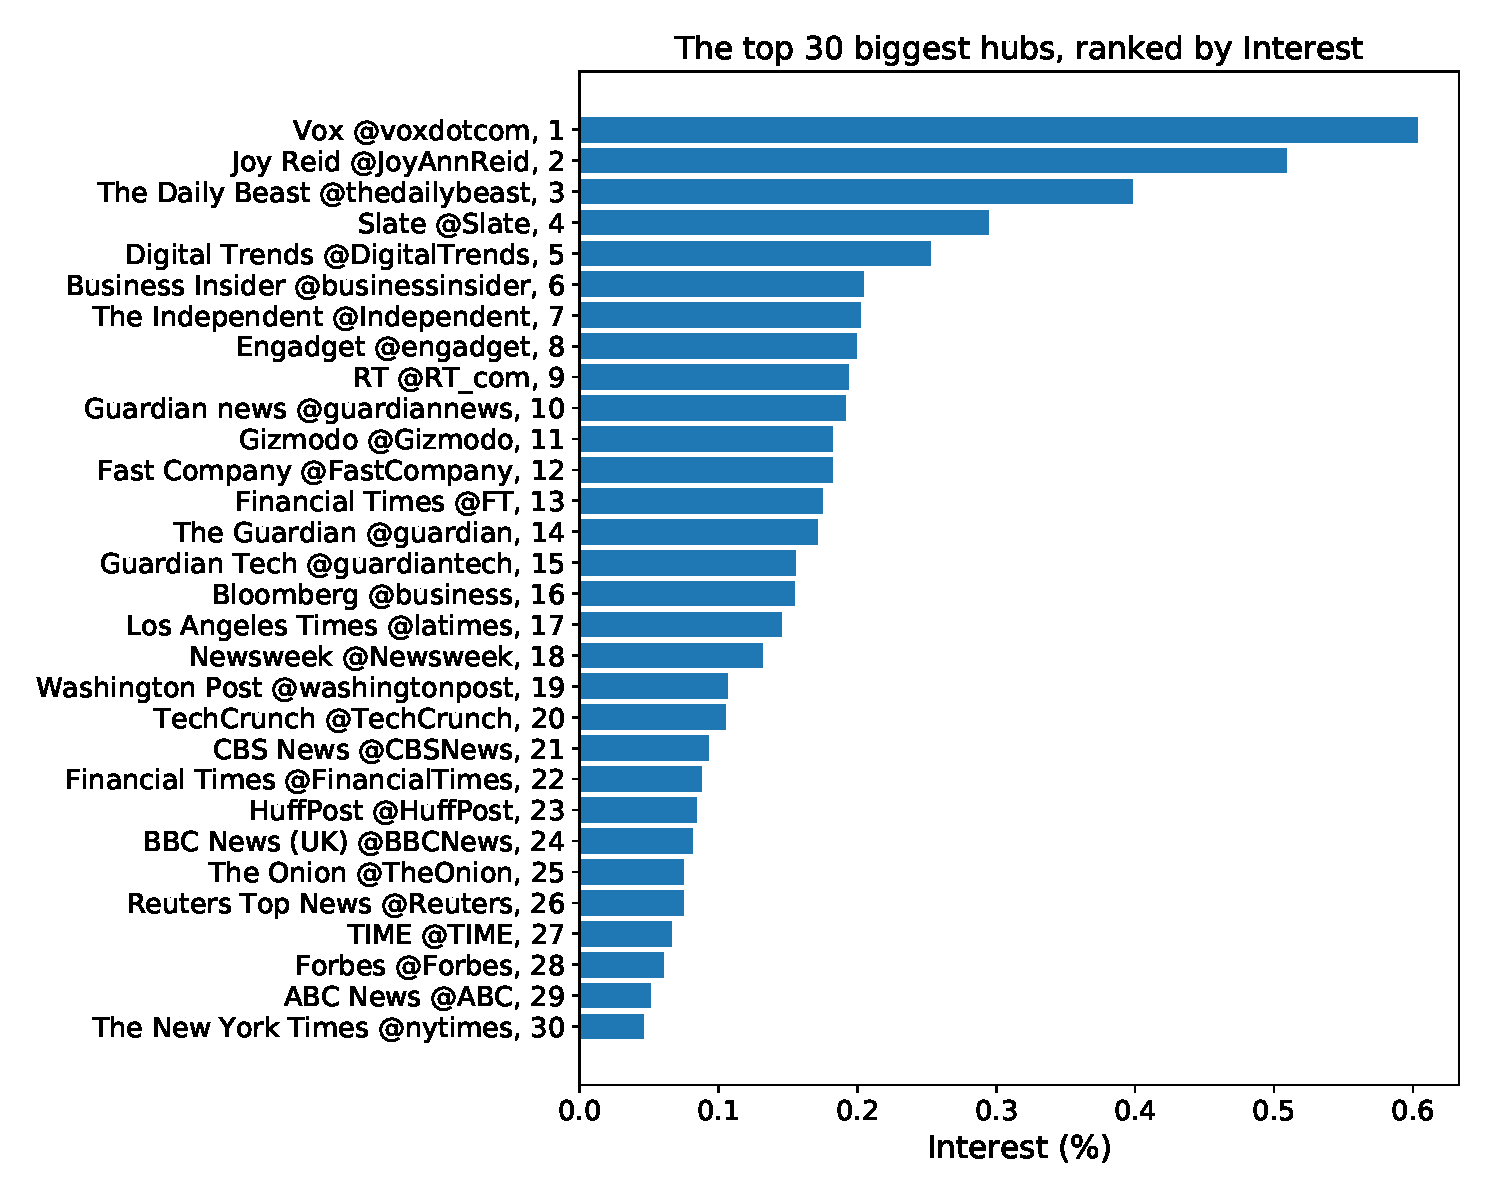
\includegraphics[width=\textwidth]{../../scripts/network_analysis/imgs/hubs_interest.pdf}            
      \caption{}
%      \label{fig:path_comparison}
    \end{figure}
    
\section{Italian sub network}
\begin{minipage}[b]{0.5\textwidth}
   \centering
    \begin{figure}[H]
      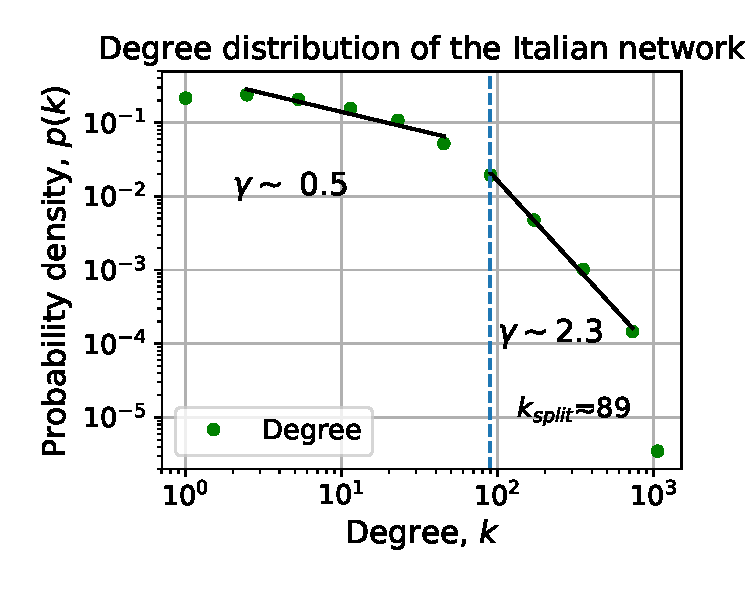
\includegraphics[width=\textwidth]{../../scripts/network_analysis/imgs/tot_degree_distribution_ita.pdf}            
          \caption{Shortest paths computation time by number of pairs}
      \label{fig:path_time}
\end{figure}
\end{minipage}
\begin{minipage}[b]{0.5\textwidth}
  \begin{figure}[H]
  \centering
      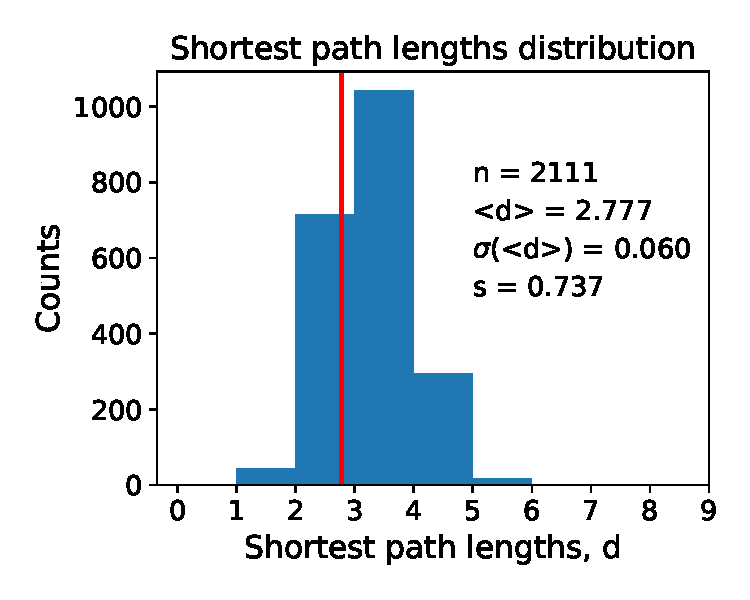
\includegraphics[width=\textwidth]{../../scripts/network_analysis/imgs/paths_hist_ita.pdf}            
        \caption{Shortest paths distribution}
\end{figure}
\end{minipage}


    \chapter{Spreading} % (fold)
\label{cha:spreading}

In this chapter we'll describe the results we obtained by applying the \textbf{SI}, \textbf{SIS}, \textbf{SIR},
and \textbf{Threshold} diffusion models both on the crawled data and on the synthetic graphs (Erdős–Rényi and
Barabási–Albert) generated from the original one. In each section, a comparison between the three networks will be
provided along with some details on the implementation of the tests of every model.

\section{SI model} % (fold)
\label{sec:si_model}
    \begin{figure}[H]
        \centering
        \begin{subfigure}{0.45\textwidth}
            \resizebox{\textwidth}{!}{
                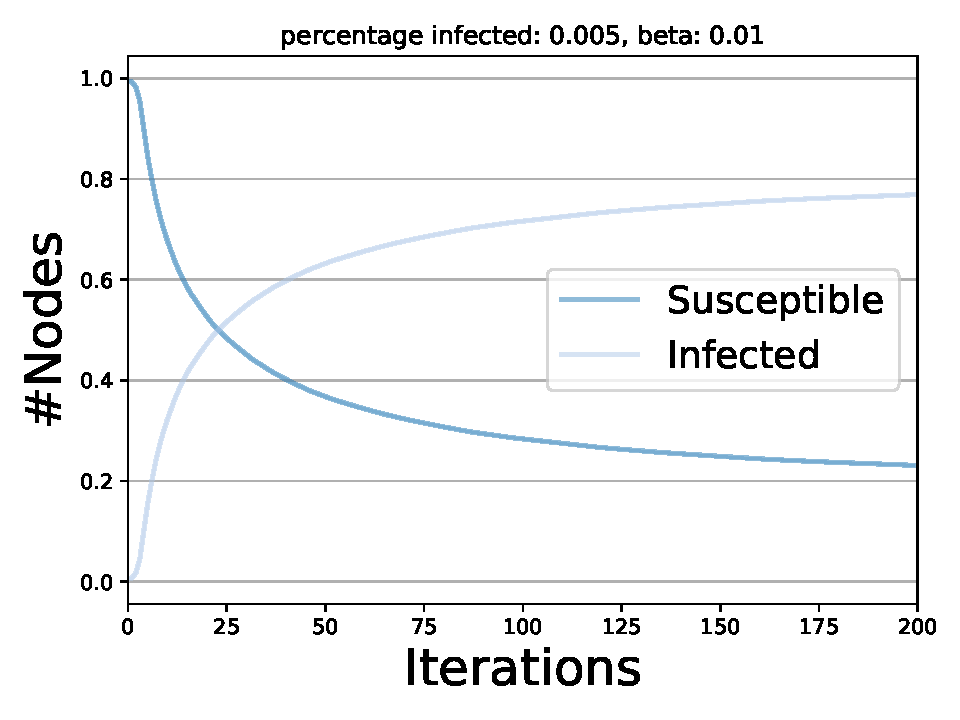
\includegraphics{images/spreading/si/diffusion.pdf}

            }
            \caption{}
            \label{diff_si}
        \end{subfigure}
        \begin{subfigure}{0.45\textwidth}
            \resizebox{\textwidth}{!}{
                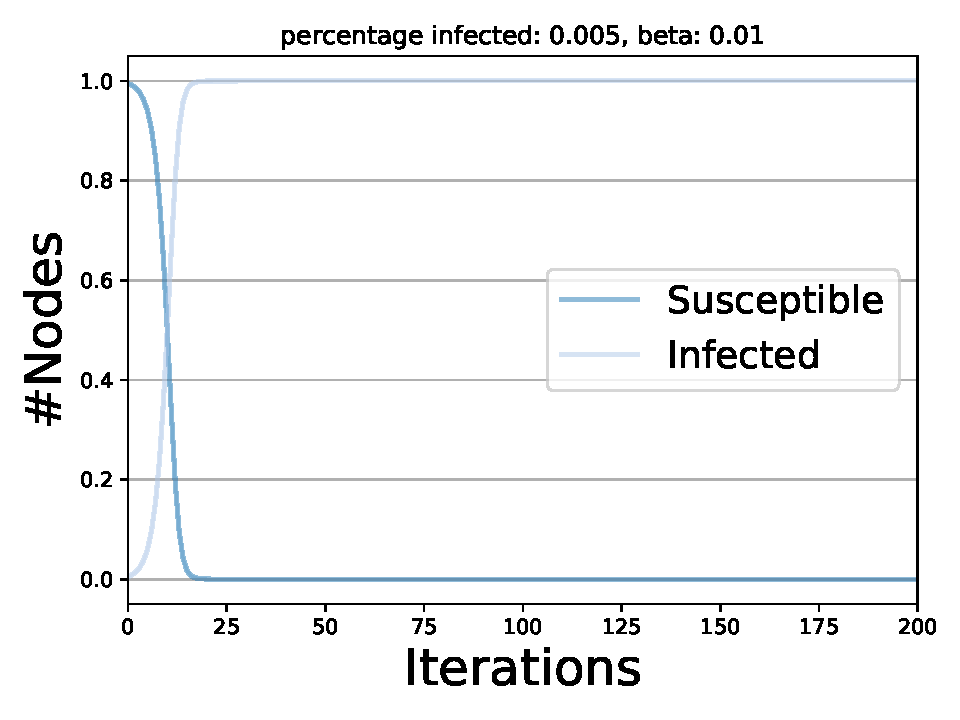
\includegraphics{images/spreading/si/diffusion_er.pdf}
            }
            \caption{}
            \label{diff_si_er}
        \end{subfigure}
        \begin{subfigure}{0.45\textwidth}
            \resizebox{\textwidth}{!}{
                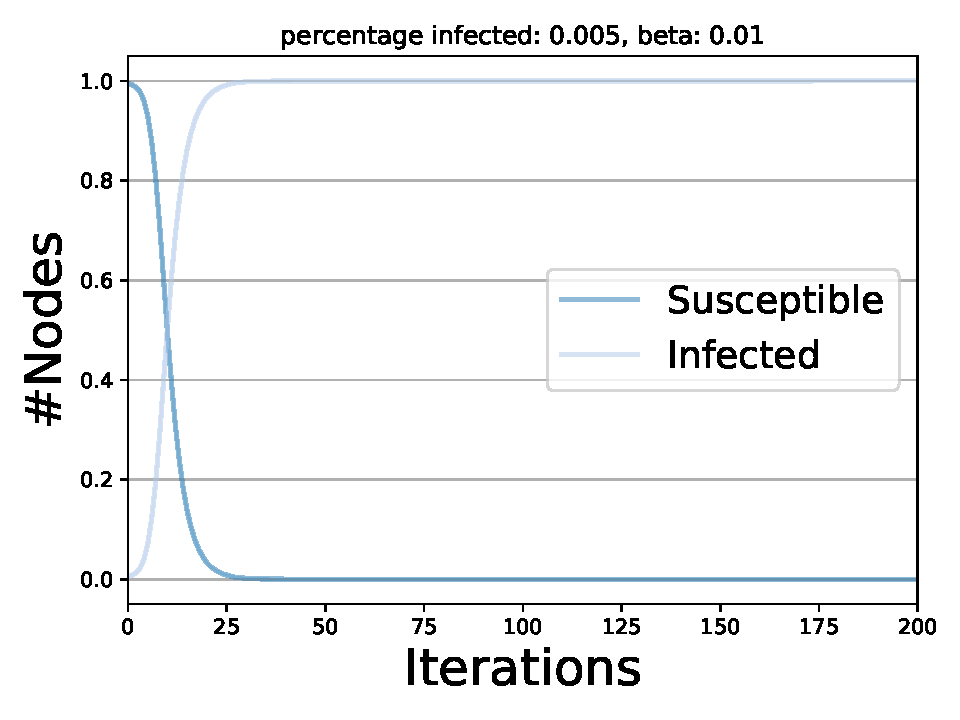
\includegraphics{images/spreading/si/diffusion_ba.pdf}
            }
            \caption{}
            \label{diff_si_ba}
        \end{subfigure}
        \begin{subfigure}{0.45\textwidth}
            \resizebox{\textwidth}{!}{
                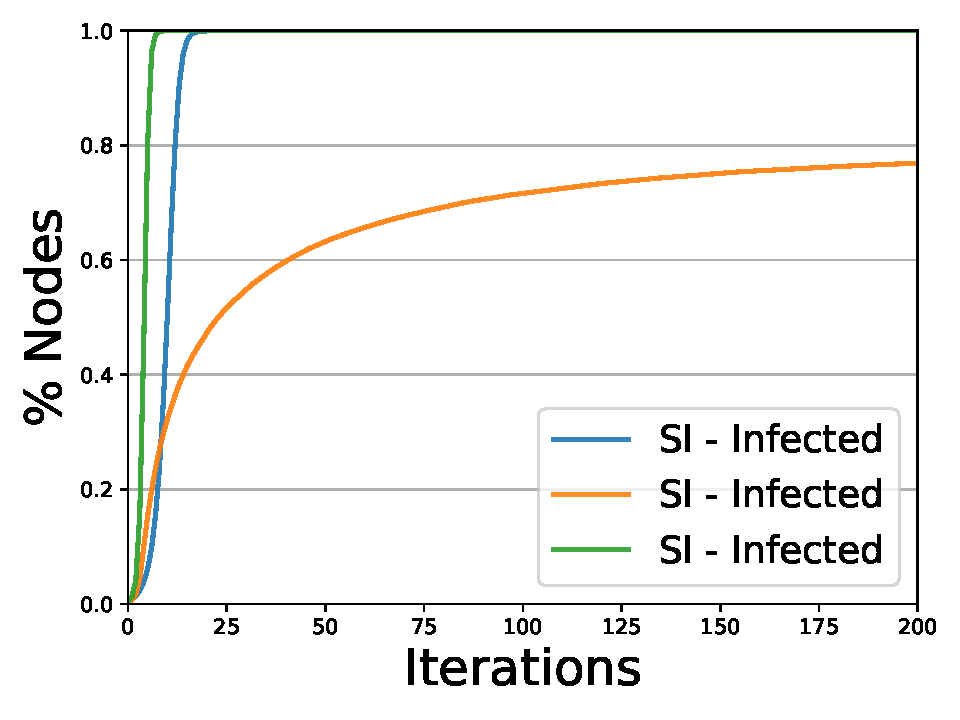
\includegraphics{images/spreading/si/trend_comparison.pdf}
            }
            \caption{}
            \label{diff_si_comparison}
        \end{subfigure}
        \caption{In Figure \ref{diff_si} we can see the diffusion graph for the original network, while in Figure
        \ref{diff_si_er} and in Figure \ref{diff_si_ba} we can see the diffusion graph for the Erdős–Rényi and
        Barabási–Albert networks, respectively. In Figure \ref{diff_si_comparison} we can see a comparison between
        the infection rate of the three networks.}
        \label{diff_si_total}
    \end{figure}
    For the \textbf{Susceptible-Infected} model we've started with a $0.005\%$ of the total population ($3$ nodes)
    of each network being infected, and we've choosed a value of $0.01$ for the infection rate $\beta$. As you can
    see from Figure \ref{diff_si_total}, the original network is the only one that doesn't reach the saturation
    regime, while the other networks reach it within the first $25$ iterations of the model. This is due to the fact
    that both the Erdős–Rényi and the Barabási–Albert network are extremely connected, hence it is more easy for the
    infection to spread among the nodes.

% section si_model (end)

\section{SIS model} % (fold)
\label{sec:sis_model}
    \begin{figure}[H]
        \centering
        \begin{subfigure}{0.45\textwidth}
            \resizebox{\textwidth}{!}{
                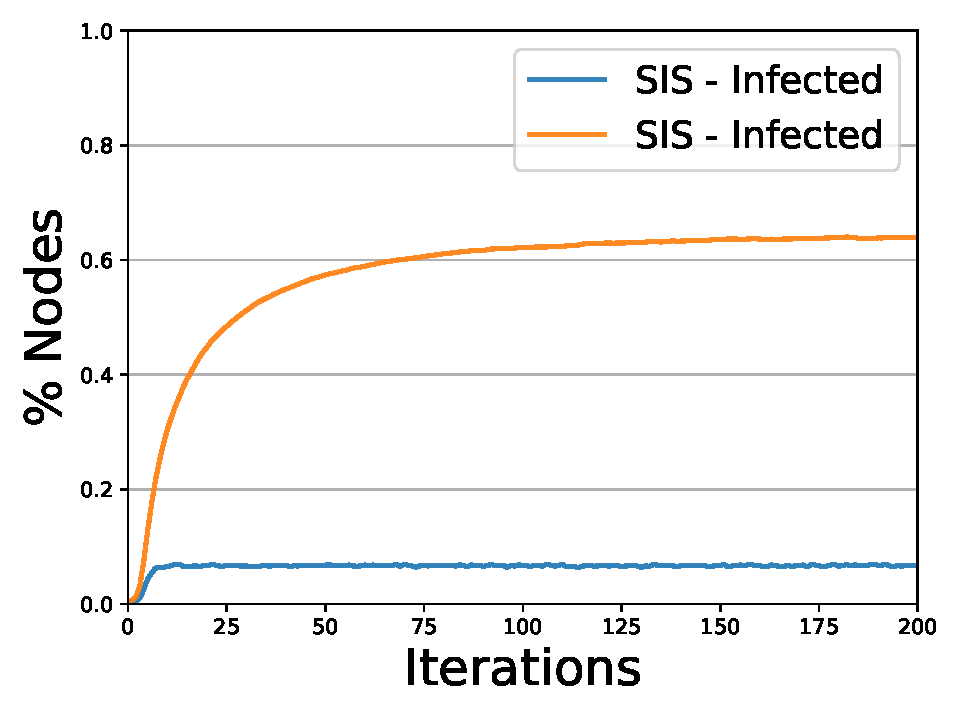
\includegraphics{images/spreading/sis/diffusion_original_comparison.pdf}
            }
            \caption{}
            \label{diff_sis}
        \end{subfigure}
        \begin{subfigure}{0.45\textwidth}
            \resizebox{\textwidth}{!}{
                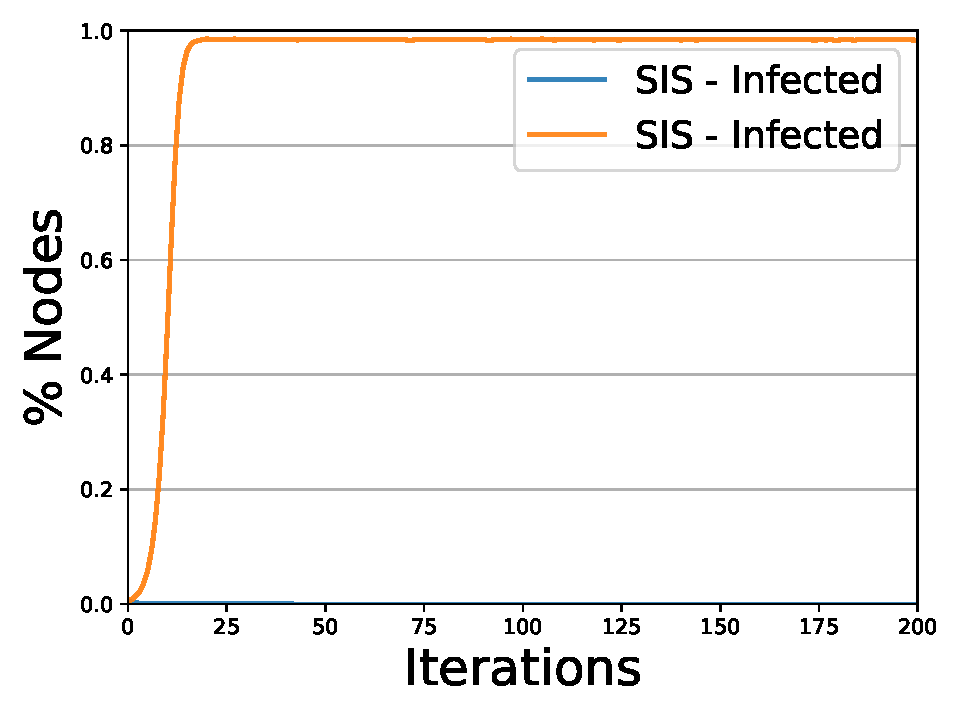
\includegraphics{images/spreading/sis/diffusion_er_comparison.pdf}
            }
            \caption{}
            \label{diff_sis_er}
        \end{subfigure}
        \begin{subfigure}{0.45\textwidth}
            \resizebox{\textwidth}{!}{
                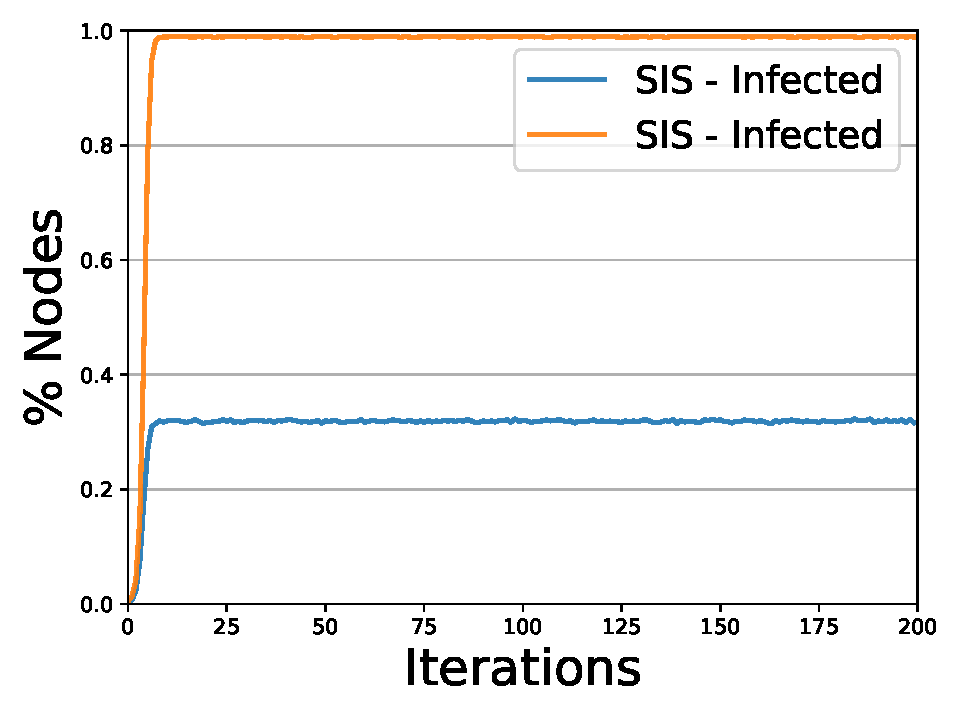
\includegraphics{images/spreading/sis/diffusion_ba_comparison.pdf}
            }
            \caption{}
            \label{diff_sis_ba}
        \end{subfigure}
        \caption{In Figure \ref{diff_sis} we can see the comparison between the endemic state, in orange, and the
        disease free state, in blue, for the original network. The same comparison can be observed for the
        Erdős–Rényi and the Barabási–Albert network, respectively, in Figure \ref{diff_sis_er} and
        \ref{diff_sis_ba}}
        \label{diff_sis_total}
    \end{figure}
    For the \textbf{Susceptible-Infected-Susceptible} model, thanks to the introduction of the recovery rate $\mu$,
    we can model two possible outcomes for the epidemic: the \textbf{endemic state}, characterized by a low recovery
    rate and by the fraction of infected individuals that follows a logistic curve similar to the one observed for
    the SI model, for which $\mu < \beta\langle k \rangle$, and the \textbf{disease free} state, characterized by a
    sufficiently high recovery rate, for which $\mu > \beta\langle k \rangle$. A comparison between this two states
    is represented for every network in Figure \ref{diff_sis_total}.

% section sis_model (end)

\section{SIR model} % (fold){}
\label{sec:sir_model}
    The key characteristic of the \textbf{Susceptible-Infected-Recovered} model consist in introducing the
    probability $\gamma$ for the individuals to recover from the disease and hence to be "removed" from the
    population instead of returning to the susceptible state. We have choosen to test this model either for the case
    in which $\gamma$ is smaller than $\beta$ and the other way around. The graphs representing this different
    situations for all the three networks are visible in Figure \ref{diff_sir_total}.
    \begin{figure}
        \begin{subfigure}{0.33\textwidth}
            \resizebox{\textwidth}{!}{
                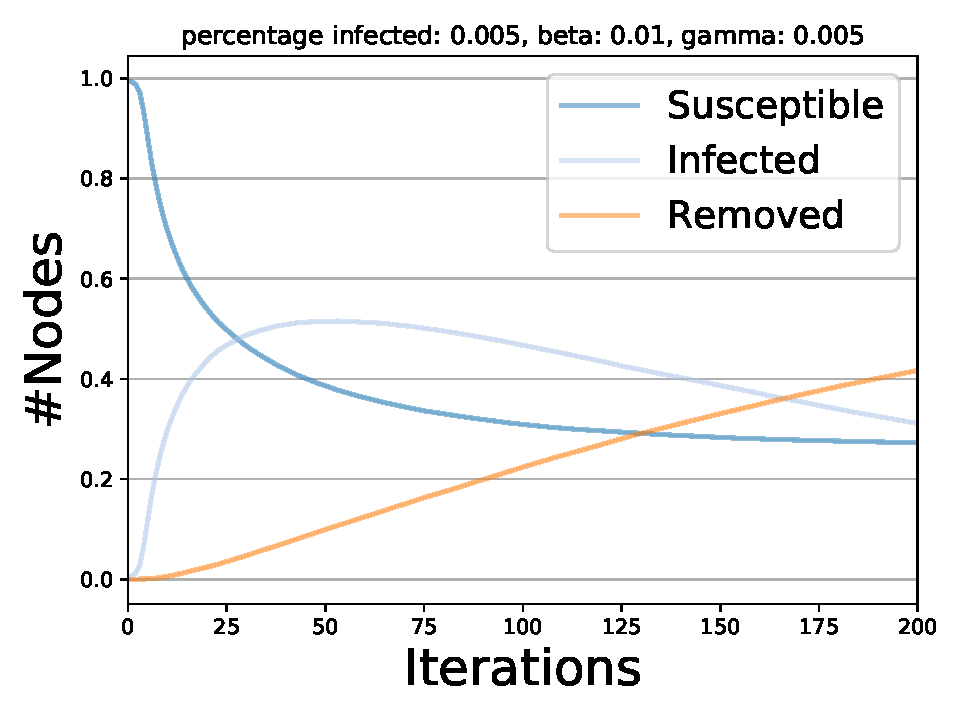
\includegraphics{images/spreading/sir/diffusion_smaller.pdf}
            }
            \caption{}
            \label{diff_sir_smaller}
        \end{subfigure}
        \begin{subfigure}{0.33\textwidth}
            \resizebox{\textwidth}{!}{
                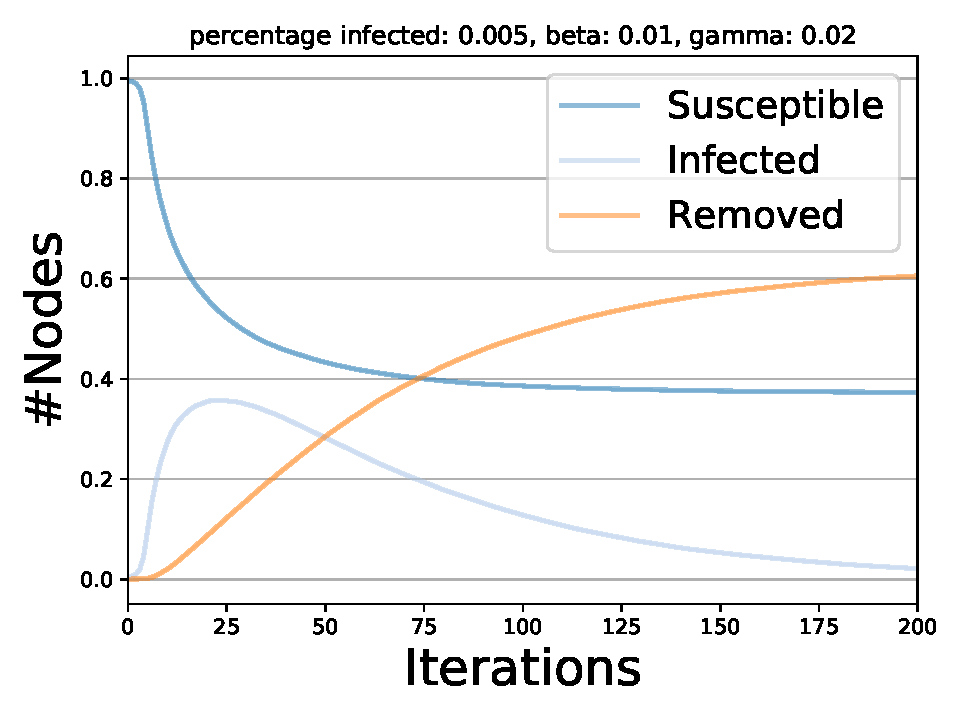
\includegraphics{images/spreading/sir/diffusion_greater.pdf}
            }
            \caption{}
            \label{diff_sir_greater}
        \end{subfigure}
        \begin{subfigure}{0.33\textwidth}
            \resizebox{\textwidth}{!}{
                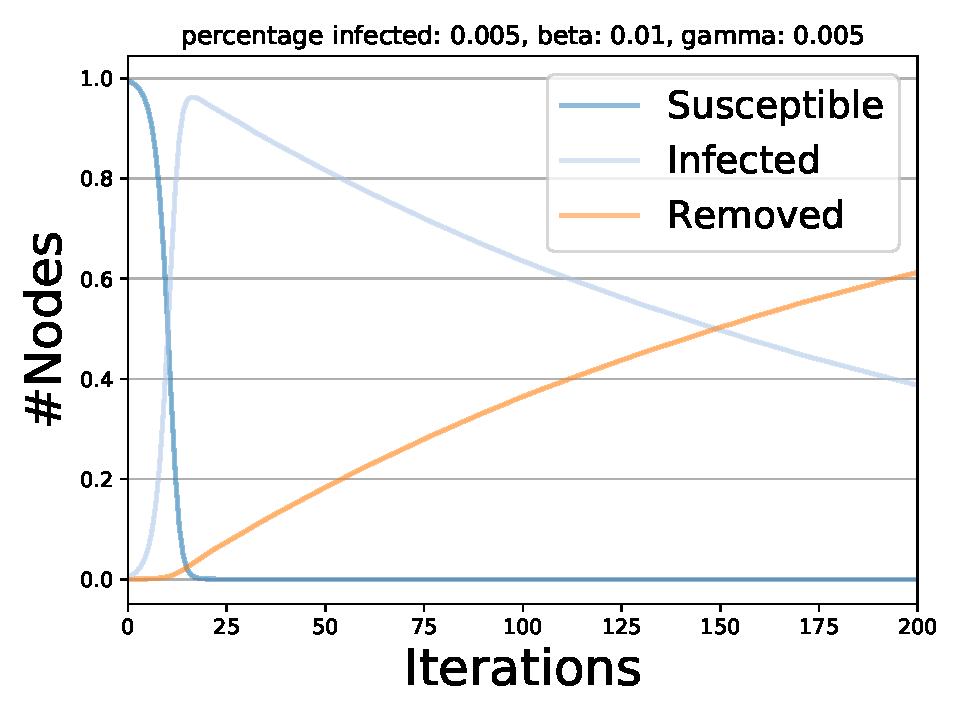
\includegraphics{images/spreading/sir/diffusion_er_smaller.pdf}
            }
            \caption{}
            \label{diff_sir_er_smaller}
        \end{subfigure}
        \begin{subfigure}{0.33\textwidth}
            \resizebox{\textwidth}{!}{
                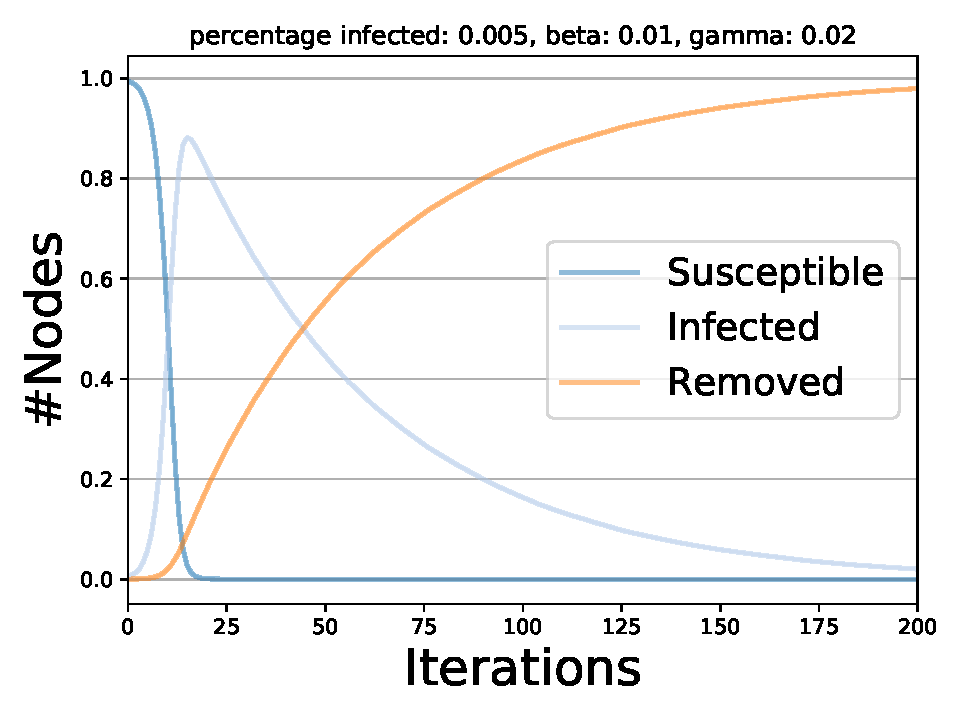
\includegraphics{images/spreading/sir/diffusion_er_greater.pdf}
            }
            \caption{}
            \label{diff_sir_er_greater}
        \end{subfigure}
        \begin{subfigure}{0.33\textwidth}
            \resizebox{\textwidth}{!}{
                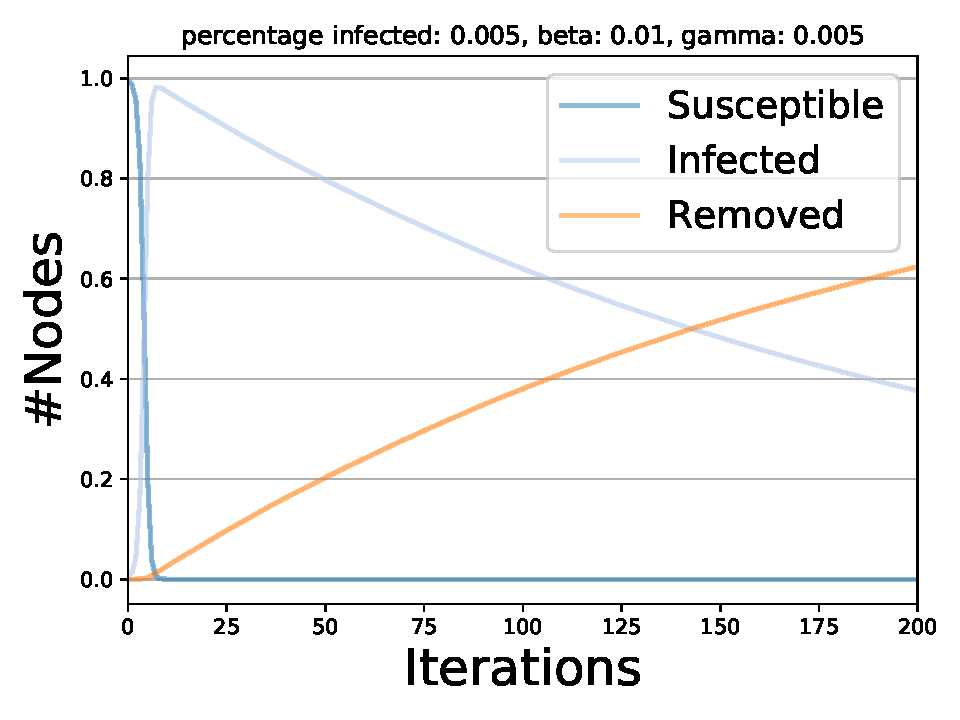
\includegraphics{images/spreading/sir/diffusion_ba_smaller.pdf}
            }
            \caption{}
            \label{diff_sir_ba_smaller}
        \end{subfigure}
        \begin{subfigure}{0.33\textwidth}
            \resizebox{\textwidth}{!}{
                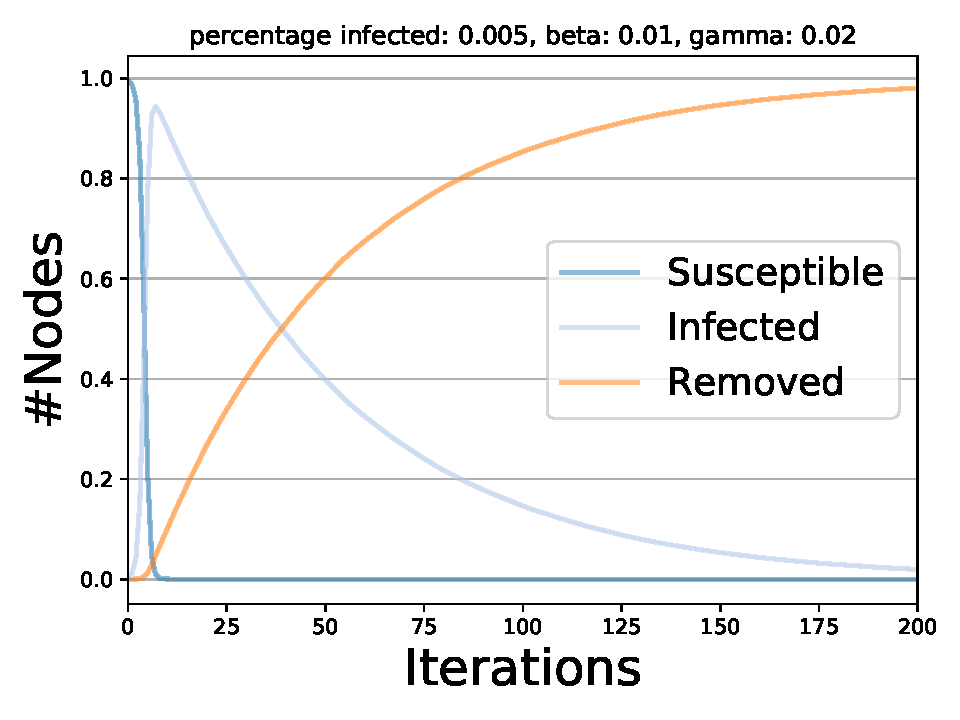
\includegraphics{images/spreading/sir/diffusion_ba_greater.pdf}
            }
            \caption{}
            \label{diff_sir_ba_greater}
        \end{subfigure}
        \caption{In Figure \ref{diff_sir_smaller} and \ref{diff_sir_greater} we can see the representation of the
        diffusion on the original network both for the case in which $\gamma$ is smaller than $\beta$ and the other
        way around. The same kind of representation is plotted for the Erdős–Rényi network in Figure
        \ref{diff_sir_er_smaller} and \ref{diff_sir_er_greater} and for the Barabási–Albert network in Figure
        \ref{diff_sir_ba_smaller} and \ref{diff_sir_ba_greater}.}
        \label{diff_sir_total}
    \end{figure}

% section sir_model (end)

\section{Threshold model} % (fold)
\label{sec:threshold_model}
    Finally we describe the application of the \textbf{Threshold model} both on the original network and the
    synthetic ones. In order to test this model we've choosen to apply a threshold $\tau$ eguals to $0.10$, the
    diffusion of the infection for this model is represented in Figure \ref{diff_thr_total}. As we can see, for the
    original network we have that almost all the nodes become infected within the first $20$ model's iterations,
    due to the fact that the value choosen for the threshold results to be sufficient for the spreading of the
    infection. If we change the threshold's value, this time using $0.20$, we can observe that the
    original network become immune to the infection, thanks to its internal structure. We can observe
    the same immunity in the Erdős–Rényi and Barabási–Albert network for the original threshold's value.
    \begin{figure}[H]
        \centering
        \begin{subfigure}{0.33\textwidth}
            \resizebox{\textwidth}{!}{
                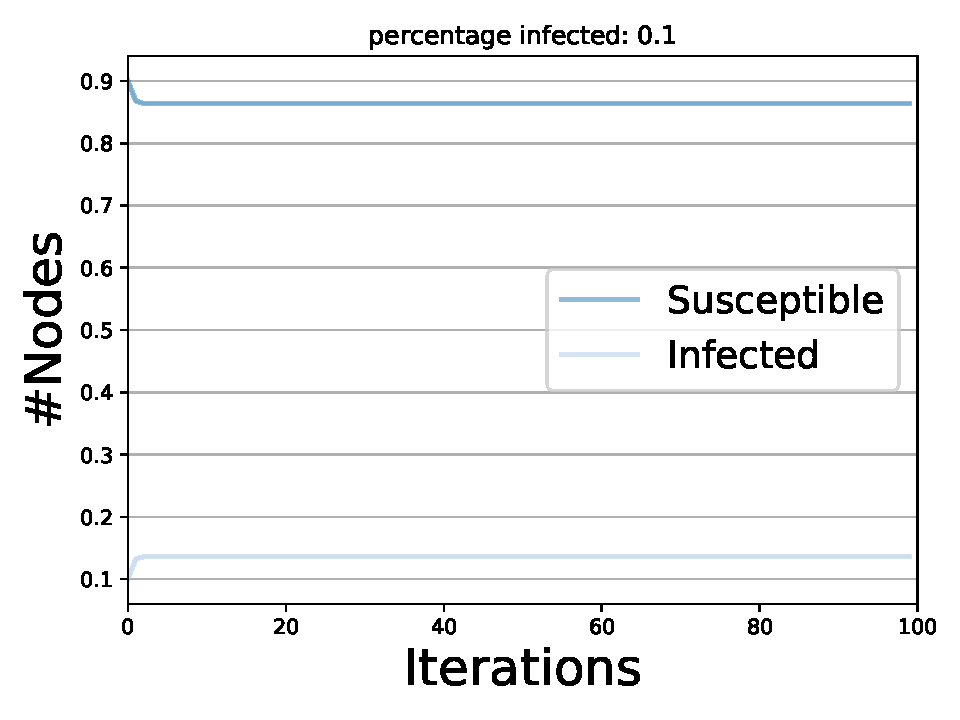
\includegraphics{images/spreading/threshold/diffusion.pdf}
            }
            \caption{}
            \label{diff_thr}
        \end{subfigure}
        \begin{subfigure}{0.33\textwidth}
            \resizebox{\textwidth}{!}{
                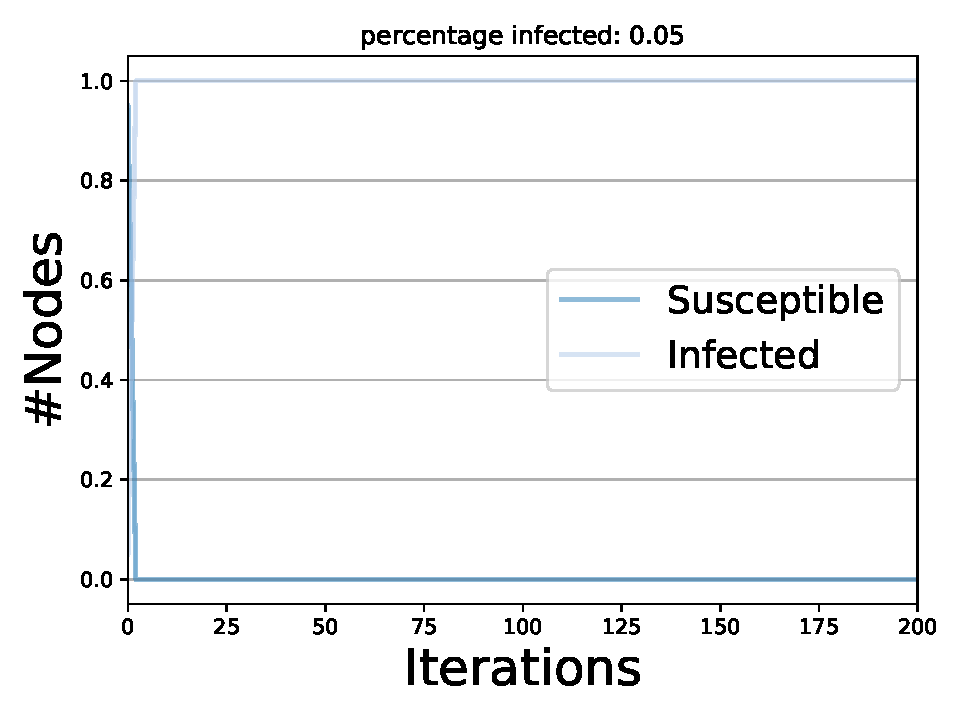
\includegraphics{images/spreading/threshold/diffusion_er.pdf}
            }
            \caption{}
            \label{diff_thr_er}
        \end{subfigure}
        \begin{subfigure}{0.33\textwidth}
            \resizebox{\textwidth}{!}{
                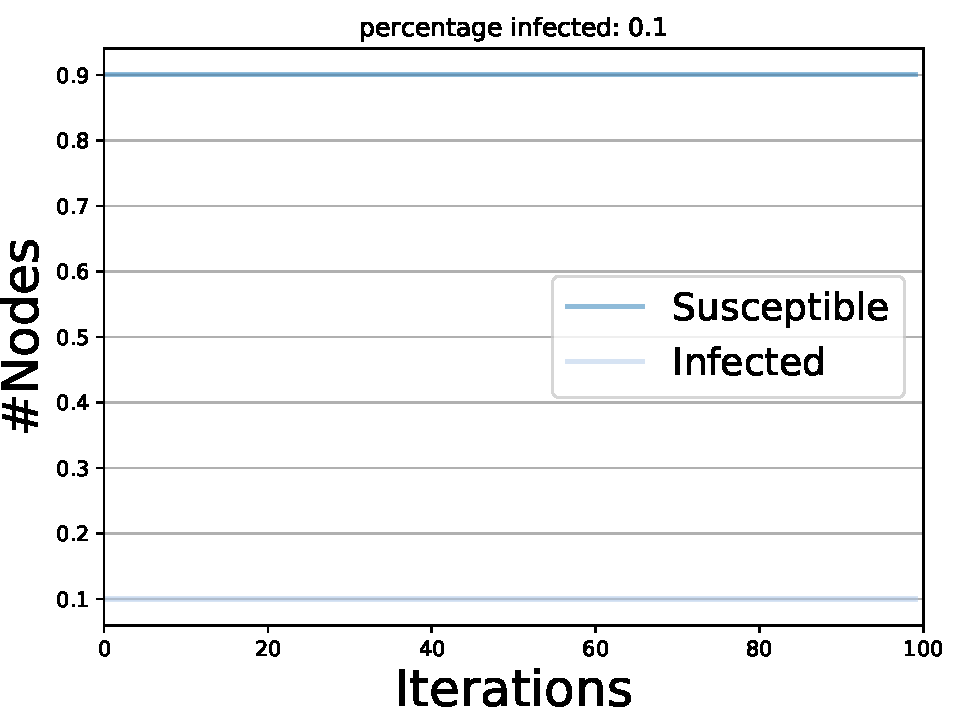
\includegraphics{images/spreading/threshold/diffusion_ba.pdf}
            }
            \caption{}
            \label{diff_thr_ba}
        \end{subfigure}
        \begin{subfigure}{0.33\textwidth}
            \resizebox{\textwidth}{!}{
                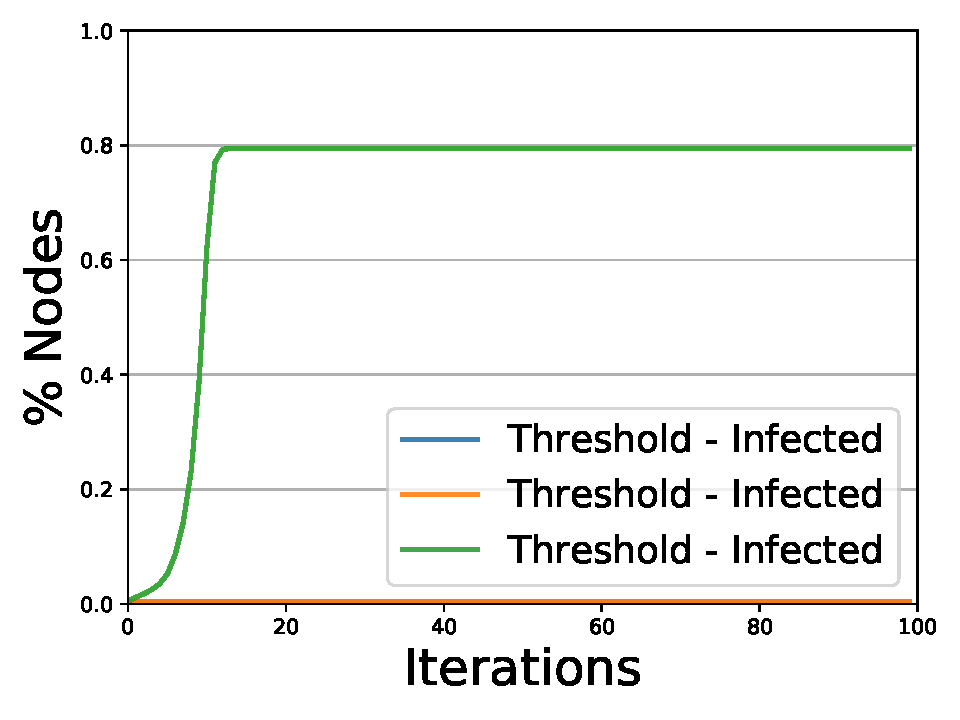
\includegraphics{images/spreading/threshold/trend_comparison.pdf}
            }
            \caption{}
            \label{diff_thr_comparison}
        \end{subfigure}
        \caption{In Figure \ref{diff_thr} is represented the diffusion of the infection for the original network,
        while in Figure \ref{diff_thr_er} and \ref{diff_thr_ba} are represented the cases for the Erdős–Rényi and
        the Barabási–Albert network, respectively. A comparison between the three networks is represented in Figure
        \ref{diff_thr_comparison}.}
        \label{diff_thr_total}
    \end{figure}

% section threshold_model (end)

% chapter spreading (end)


    \chapter{Communities discovery} % (fold)
\label{cha:communities_discovery}

In this chapter we'll provide the results obtained by applying \textbf{K-Clique}, \textbf{Label Propagation},
\textbf{Louvain}, \textbf{Girvan-Newman} and \textbf{Demon} to a sample of $1000$ nodes taken from the original
network. We've chosen to sample the crawled data in order to ease the application of the various algorithms.
Each partition is evaluated by applying an implementation of the scoring functions listed in
\cite{comm_ground_truth}, and, for each algorithm, the results are represented in a table. Together with the
results of the scoring functions are also provided the total number of communities discoverd (Communities), the
number of nodes in the smallest/biggest community (Smallest/Biggest), the hashtags utilized in the biggest
community (Tags) and finally the languages of the users in the biggest community (Langs).

\section{K-Clique} % (fold)
\label{sec:k_clique}
    We have chosen to apply the \textbf{K-Clique} algorithm, described in \cite{k_clique}, to the sample using
    three different values for $k$: $3$, $4$ and $5$, respectively. The results are represented in Table
    \ref{kclique}. As we can see, even if the result is not so good, the best partition is obtained by using $k$
    eguals to $3$, which returns a low modularity partition composed by low degree nodes. It is interesting to
    note that all the biggest partitions returned by the various applications of the algorithm are composed only
    by english speaking users.

    \begin{table}[H]
        \centering
        \begin{subtable}{\textwidth}
            \resizebox{\textwidth}{!}{
                \begin{tabular}{| c | c | c | c | c | c | c | c | c | c |}
                    \hline
                    K & Communities & Biggest & Smallest & Modularity & Conductance & IED & AND &  Tags &
                    Langs \\
                    \hline
                    3 & 29 & 51 & 3 & 0.14 & 0.62 & 0.20 & 2.72 & zuckerberg,
                    cambridgeanalytica, deletefacebook, facebook, facebookgate & English, Deutsch \\
                    \hline
                    4 & 13 & 14 & 4 & 0.020 & 0.68 & 0.21 & 4.23 & cambridgeanalytica, deletefacebook, facebook
                    & English \\
                    \hline
                    5 & 5 & 12 & 5 & 0.011 & 0.63 & 0.23 & 4.83 & cambridgeanalytica, deletefacebook, facebook
                    & English \\
                    \hline
                \end{tabular}
            }
        \end{subtable}
        \caption{Evaluation of the partitions obtained by the application of the K-Clique algorithm.}
        \label{kclique}
    \end{table}

% section k_clique (end)

\section{Label Propagation} % (fold)
\label{sec:label_propagation}
    In Table \ref{labelprop} are represented the results of the application of the \textbf{Label Propagation}
    algorithm, described in \cite{label_propagation}. According to the modularity score the partition provided by
    this algorithm represent a good subdivision of the original network, even if it is composed for the vast
    majority by small communities, as suggested by the high number of communities and the low value for the
    Average Node Degree score. As for the kclique algorithm, it is interesting to note that the biggest community
    is composed only by english speaking users.

    \begin{table}[H]
        \centering
        \begin{subtable}{\textwidth}
            \resizebox{\textwidth}{!}{
                \begin{tabular}{| c | c | c | c | c | c | c | c | c |}
                    \hline
                    Communities & Biggest & Smallest & Modularity & Conductance & IED & AND &  Tags & Langs \\
                    \hline
                    1278 & 136 & 1 & 0.68 & 0.28 & 0.19 & 1.38 & cambridgeanalytica,
                    deletefacebook, privacy, zuckerberg, facebook, facebookgate & Various  \\
                    \hline
                \end{tabular}
            }
        \end{subtable}
        \caption{Evaluation of the partition obtained by the application of the Label Propagaion algorithm.}
        \label{labelprop}
    \end{table}

% section label_propagation (end)

\section{Louvain} % (fold)
\label{sec:louvain}
    The application of the \textbf{Louvain}, described in \cite{louvain}, along with the last iteration of the
    Girvan-Newman algorithm, returns the best partition among all the partitions returned by the other algorithms.
    The results of its application are represented in Table \ref{louvain}. As for the Label Propagation algorithm,
    this partition also is composed by an high number of small communities, composed by nodes with degree betweem
    $1$ and $2$.

    \begin{table}[H]
        \centering
        \begin{subtable}{\textwidth}
            \resizebox{\textwidth}{!}{
                \begin{tabular}{| c | c | c | c | c | c | c | c | c |}
                    \hline
                    Communities & Biggest & Smallest & Modularity & Conductance & IED & AND &  Tags & Langs \\
                    \hline
                    1193 & 133 & 1 & 0.76 & 0.042 & 0.17 & 1.60 & cambridgeanalytica,
                    deletefacebook, privacy, zuckerberg, facebook, facebookgate & Various \\
                    \hline
                \end{tabular}
            }
        \end{subtable}
        \caption{Evaluation of the partition obtained by the application of the Louvain algorithm.}
        \label{louvain}
    \end{table}

% section louvain (end)

\section{Girvan-Newman} % (fold)
\label{sec:girvan_newman}
    For the \textbf{Girvan-Newman} algorithm, described in \cite{girvan_newman}, we've decided to record
    the results of $5$ iterations over the sample network. The results are represented in Table
    \ref{girvan_newman}. As you can see, the first iteration returns a very poor partition, with a low modularity
    score, due to the fact that the edge with the highest betweenness centrality in the starting sample network
    doesn't provide a good grade of separation among the nodes of the network. With the second iteration, and the
    ones after that, there is a consistent improvement either in the modularity score and in the other measures.
    \begin{table}[H]
        \centering
        \begin{subtable}{\textwidth}
            \resizebox{\textwidth}{!}{
                \begin{tabular}{| c | c | c | c | c | c | c | c | c | c |}
                    \hline
                    Iteration & Communities & Biggest & Smallest & Modularity & Conductance & IED & AND &  Tags &
                    Langs \\
                    \hline
                    1 & 1181 & 703 & 1 & 0.17 & 0.00098 & 0.22 & 1.23 & cambridgeanalytica,
                    deletefacebook, privacy, zuckerberg, facebook, facebookgate & Various \\
                    \hline
                    2 & 1182 & 659 & 1 & 0.24 & 0.0019 & 0.21 & 1.27 & cambridgeanalytica,
                    deletefacebook, privacy, zuckerberg, facebook, facebookgate & Various \\
                    \hline
                    3 & 1183 & 588 & 1 & 0.38 & 0.0048 & 0.21 & 1.35 & cambridgeanalytica, deletefacebook, privacy,
                    zuckerberg, facebook, facebookgate & Various \\
                    \hline
                    4 & 1184 & 575 & 1 & 0.40 & 0.0081 & 0.20 & 1.34 & cambridgeanalytica, deletefacebook, privacy,
                    zuckerberg, facebook, facebookgate & Various \\
                    \hline
                    5 & 1185 & 458 & 1 & 0.57 & 0.011 & 0.20 & 1.40 & zuckerberg, cambridgeanalytica, deletefacebook,
                    facebook, facebookgate & Various \\
                    \hline
                \end{tabular}
            }
        \end{subtable}
        \caption{Evaluation of the partition obtained by the application of the Girvan-Newman algorithm.}
        \label{girvan_newman}
    \end{table}

    In general, the partitions returned by the five iterations of the algorithms are all composed by an high number
    of small communities.

% section girvan_newman (end)

\section{Demon} % (fold)
\label{sec:demon}
    Finally in Table \ref{demon} we provide the results of the application of the \textbf{Demon} algorithm,
    described in \cite{demon}, that we tested for three different values of $\epsilon$, $0.25$, $0.50$ and $0.75$,
    respectively. In general, the three partitions are not so good from the point of view of the modularity score,
    with the first application of the algorithm beign the best among the three
    Contrary to the results obtained by the application of the other algorithms, the partitions for the Demon
    algorithm are all composed by a small number of communities, with the last one being the "denser" one, which
    are composed by nodes with a degree between $3$ and $4$.

    \begin{table}[H]
        \centering
        \begin{subtable}{\textwidth}
            \resizebox{\textwidth}{!}{
                \begin{tabular}{| c | c | c | c | c | c | c | c | c | c |}
                \hline
                Epsilon & Communities & Biggest & Smallest & Modularity & Conductance & IED & AND &  Tags & Langs \\
                \hline
                0.10 & 10 & 147 & 4 & 0.07 & 0.46 & 0.082 & 4.41 &
                zuckerberg, cambridgeanalytica, deletefacebook, facebook, facebookgate & Various \\
                \hline
                0.25 & 11 & 63 & 4 & 0.095 & 0.44 & 0.094 & 4.31 &
                zuckerberg, cambridgeanalytica, deletefacebook, facebook, facebookgate & English, Deutsch \\
                \hline
                0.50 & 21 & 43 & 4 & 0.11 & 0.57 & 0.10 & 4.15 &
                zuckerberg, cambridgeanalytica, deletefacebook, facebook, facebookgate & English, Deutsch \\
                \hline
                0.75 & 39 & 25 & 4 & 0.62 & 0.51 & 0.12 & 3.96 &
                zuckerberg, cambridgeanalytica, deletefacebook, facebook, facebookgate & English, Deutsch \\
                \hline
                0.90 & 89 & 24 & 4 & 0.071 & 0.68 & 0.15 & 3.65 &
                zuckerberg, cambridgeanalytica, deletefacebook, facebook, facebookgate & English, Deutsch \\
                \hline
                \end{tabular}
            }
        \end{subtable}
        \caption{Evaluation of the partition obtained by the application of the Demon algorithm.}
        \label{demon}
    \end{table}

% section demon (end)

\section{Comparisons} % (fold)
\label{sec:comparisons}
    In this final section of the chapter we compare the algorithms used so far by confronting the best instances
    among the iterations provided in the past sections. The comparisons are performed by using the NF$1$ score, as
    described in \cite{rossetti2016}.

    \begin{table}[H]
        \centering
        \begin{subtable}{\textwidth}
            \resizebox{\textwidth}{!}{
                \begin{tabular}{| c | c | c | c | c | c | c | c | c |}
                    \hline
                    A1 & A2 & F1 mean & Ground Truth Communities & Identified Communities & Community Ratio &
                    Ground Truth Matched & Node Coverage & NF1 \\
                    \hline
                    K-Clique 3 & Label Propagation & 0.44 & 714.0 & 21.0 & 0.029 & 0.022 & 0.10 & 0.0076 \\
                    \hline
                    K-Clique 3 & Louvain & 0.32 & 683.0 & 21.0 & 0.031 & 0.016 & 0.10 & 0.0027 \\
                    \hline
                    K-Clique 3 & Girvan-Newman 5 & 0.25 & 677.0 & 21.0 & 0.031 & 0.012 & 0.10 & 0.0011 \\
                    \hline
                    K-Clique 3 & Demon 0.25 & 0.92 & 6.0 & 21.0 & 3.5 & 1.0 & 1.44 & 0.24 \\
                    \hline
                    Label Propagation & Louvain & 0.96 & 683.0 & 714.0 & 1.05 & 1.0 & 1.0 & 0.92 \\
                    \hline
                    Label Propagation & Girvan-Newman 5 & 0.95 & 677.0 & 714.0 & 1.06 & 1.0 & 1.0
                    & 0.90 \\
                    \hline
                    Label Propagation & Demon 0.25 & 0.38 & 6.0 & 714.0 & 119.0 & 1.0 & 14.17
                    & 0.0032 \\
                    \hline
                    Louvain & Girvan-Newman 5 & 0.99 & 677.0 & 683.0 & 1.01 & 1.0 & 1.0 & 0.98 \\
                    \hline
                    Louvain & Demon 0.25 & 0.38 & 6.0 & 683.0 & 113.83 & 1.0 & 14.17 & 0.0033 \\
                    \hline
                    Girvan-Newman 5 & Demon 0.25 & 0.36 & 6.0 & 677.0 & 112.83 & 1.0 & 14.17 & 0.0032 \\
                    \hline
                \end{tabular}
            }
        \end{subtable}
        \caption{Comparisons among the best iterations of the algorithms utilized in this chapter.}
        \label{comparisons}
    \end{table}

    In Table \ref{comparisons} we can see the comparisons among the best iterations of the algorithms utilized
    during the community discovery phase. As we can see, the best results are returned by the comparisons between
    the Label Propagation, Louvain and Girvan-Newman (fifth iteration) algorithms, since that, as we've seen in
    the past sections, they are in fact the best performing algorithms among the ones we've tested for the
    communities discovery.
% section comparisons (end)

% chapter communities_discovery (end)


    \chapter{Network robustness} % (fold)
\label{cha:network_robustness}
    In this chapter we'll provide some results about the \textbf{robustness} and \textbf{attack tolerance} of our
    network. Thaking as reference the concepts described in \cite{network_science}, we'll define the
    \textbf{critical threshold} of our network, and we'll test its robustness against attacks conducted following
    a random nodes' selection or one based on decreasing degree centrality. Finally we'll test the
    \textbf{Failure Propagation Model}, following our implementation of the model, on our network.
    \section{Critical threshold} % (fold)
    \label{sec:critical_threshold}
        As described in \cite{network_science}, we have obtained the \textbf{critical threshold}
        representing the fraction of the nodes that must be removed to break apart our network. This fraction,
        represented by $f_c$, is obtained by the following formula:

        \begin{equation*}
            f_c = 1 - \frac{1}
            {\frac{\gamma - 2}{3 - \gamma}k^{\gamma - 2}_{\mathit{min}}k^{3 - \gamma}_{\mathit{max}} \ - \  1} =
            1 - \frac{1}{1.50 * 1^{0.6} * 19073^{0.4} \ - \ 1} = 0.99
        \end{equation*}

        which, remembering that the $\gamma$ for our scale-free network corresponds to $2.6$ and that
        $k_{\mathit{min}}$ and $k_{\mathit{max}}$ are eguals to $1$ and $19073$ respectively, tells us that, in
        order to break apart our network it is mandatory to remove the $99\%$ of the nodes. Keeping in mind that
        our network is, in fact, a finite network, we can adjust the obtained result by utilizing the following
        formula, still in \cite{network_science}:

        \begin{equation*}
            f_c \approx 1 - \frac{C}{N^{\frac{3 - \gamma}{\gamma - 1}}} \approx 1.00
        \end{equation*}

        where $C = \frac{1}{\sum_{k=1}^{\infty}k^{-\gamma}}$ is a constant and $N$ represents the number of nodes
        of the network. As we can see, this new approximation tells us that in order to break apart our network the
        totality of its nodes must be removed.
    % section critical_threshold (end)
    \section{Simulation of an attack} % (fold)
    \label{sec:simulation_of_an_attack}
        In order to validate the results obtained in Section \ref{sec:critical_threshold}, here we simulate an
        attack to our network. We've chosen to simulate the remotion of $50$ nodes from the network following two
        distinct criterions: \textbf{random selection} and \textbf{degree centraility} (decreasing order). For every
        criterion we've monitored the fragmentation of the connected components.

        \begin{figure}[H]
            \centering
            \begin{subfigure}{0.45\textwidth}
                \resizebox{\textwidth}{!}{
                    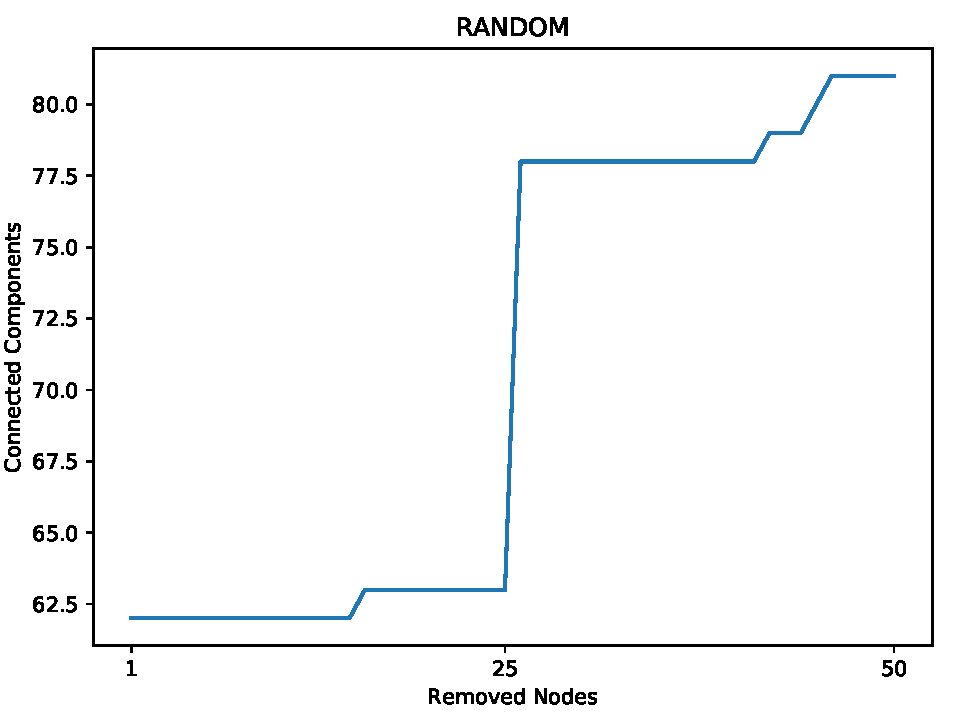
\includegraphics{images/robustness/test_cc_on_random.pdf}
                }
                \caption{}
                \label{test_cc_on_random}
            \end{subfigure}
            \begin{subfigure}{0.45\textwidth}
                \resizebox{\textwidth}{!}{
                    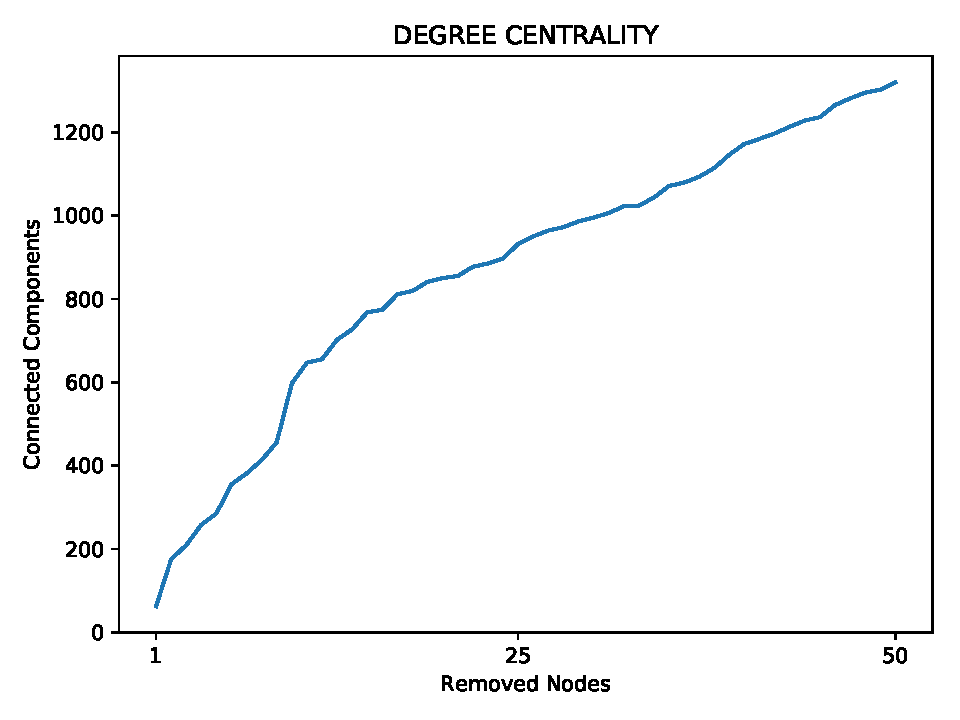
\includegraphics{images/robustness/test_cc_on_degree_centrality.pdf}
                }
                \caption{}
                \label{test_cc_on_degree_centrality}
            \end{subfigure}
            \caption{In Figure \ref{test_cc_on_random} we can see the fragmentation of the connected components
            during the remotion based on a randomic choice, while in Figure \ref{test_cc_on_degree_centrality} we
            can see the same fragmentation, but this time based on decreasing degree centraility.}
            \label{test_cc}
        \end{figure}

        As we can see, for the randomic choice of the nodes to be removed, the structure of the network is barely
        altered. After the random remotion of $50$ nodes, the original $62$ connected components became slightly
        more than $80$. For the remotion of the nodes based on decreasing degree centrality there is, as expected,
        a different situation. This kind of criterion guarantees that the original structure of the network is
        broken apart more easily, because the original network's hubs are removed one by one in decreasing order.
    % section simulation_of_an_attack (end)
    \section{Simulation of a Failure Propagation Model} % (fold)
    \label{sec:simulation_of_a_failure_propagation_model}
        To test more the robustness of our network, we've written the code in order to implement (and test) the
        \textbf{Failure Propagation Model}, as described in \cite{network_science}. In Figure \ref{fail_prop_model}
        you can see some iterations of the model in which we used different values for the $\varphi$ parameter.

        \begin{figure}[H]
            \centering
            \begin{subfigure}{0.50\textwidth}
                \resizebox{\textwidth}{!}{
                    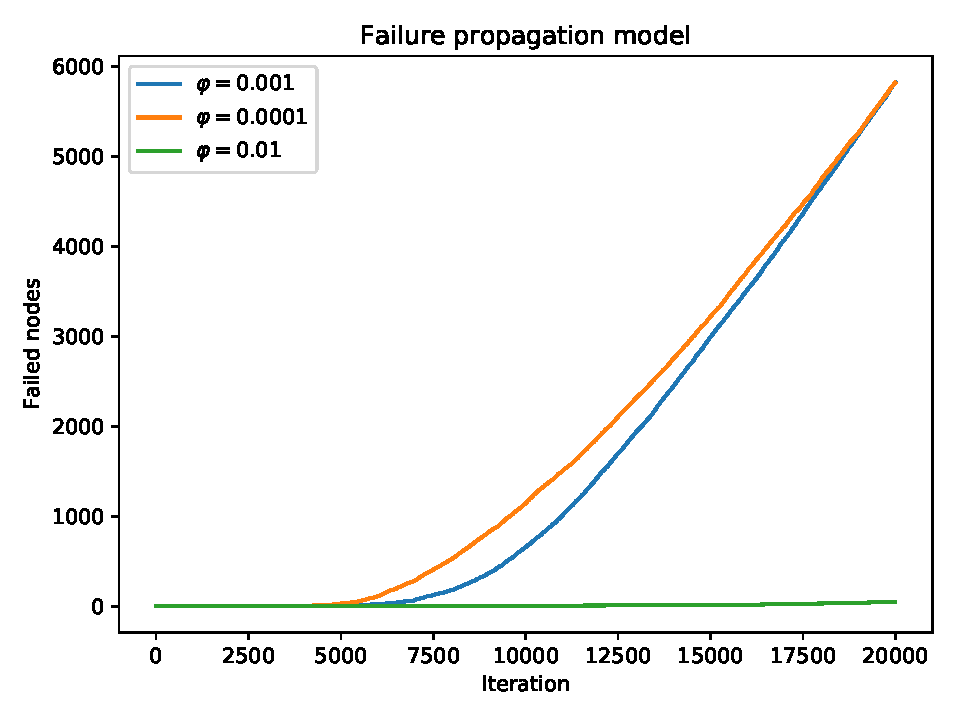
\includegraphics{images/robustness/failure_propagation_model.pdf}
                }
            \end{subfigure}
            \caption{The test for the Failure Propagation Model was conducted over $20000$ iterations.}
            \label{fail_prop_model}
        \end{figure}

        We can see that, as expected, the network doesn't accuse the failure propagation for $\varphi$ eguals to
        $0.01$, in which less than $30$ nodes failed. For the smaller values of $\varphi$ we can see that the
        situation is different, with a greater amount of nodes which fail over the iterations.
    % section simulation_of_a_failure_propagation_model (end)
% chapter network_robustness (end)


    \chapter{Summary}


\printbibliography[title={References}]


\end{document}
